
\documentclass[11pt,fleqn]{article}
\usepackage[margin=1in,top=1in,bottom=1in]{geometry}
\usepackage{mathtools}
\usepackage{longtable}
\usepackage{enumitem}
\usepackage{hyperref}
\usepackage[dvips]{graphics}
\usepackage[table]{xcolor}
\usepackage{amssymb}
\usepackage{subfig}
\usepackage{booktabs}
\usepackage{tikz}
\usepackage{pdflscape}

\usepackage[normalem]{ulem}

\usepackage{multicol}
\usepackage{txfonts}
%\usepackage{amsfonts}
\usepackage{natbib}

\usepackage{gb4e}
%\usepackage{/Users/judith/Library/Latex/drs}
%\usepackage{/Users/judith/Library/Latex/avm}
\usepackage[all]{xy}
\usepackage{rotating}
\usepackage{tipa}
\usepackage{multirow}
\usepackage{authblk}
\usepackage{adjustbox}
\usepackage{array}


\newcolumntype{R}[2]{%
    >{\adjustbox{angle=#1,lap=\width-(#2)}\bgroup}%
    l%
    <{\egroup}%
}
\newcommand*\rot{\multicolumn{1}{R{90}{1em}}}% no optional argument here, please!

\newcommand{\foc}{$_{\mbox{\small F}}$}
\newcommand{\lp}{<_{\hspace*{-.1cm}p}}
\newcommand{\lnai}{<_{\hspace*{-.1cm}nai}}

\setlength{\parindent}{.8cm}
\setlength{\parskip}{0ex}
\setlength{\headsep}{0in}

\setlength{\bibsep}{0mm}
\bibpunct[:]{(}{)}{;}{a}{,}{,}

\newcommand{\yi}{\'{\symbol{16}}}
\newcommand{\nasi}{\~{\symbol{16}}}
\newcommand{\hina}{h\nasi na}
\newcommand{\ina}{\nasi na}
%\renewcommand{\abut}{$\supset$\hspace*{-0.07cm}$\subset$}
\newcommand{\tto}{t$_{top}$}
\newcommand{\wtop}{w$_{top}$}
\newcommand{\tc}{t$_c$}
\newcommand{\schwa}{\begin{sideways}e\end{sideways}}

% Semantic brackets
%\newcommand{\iss}[1]{\mbox{\protect\tiny \mbox{#1}}}
%\newcommand{\sem}[2]{\6#1\9$_\iss{#2}$} David's original
\newcommand{\6}{\mbox{$[\hspace*{-.6mm}[$}} 
\newcommand{\9}{\mbox{$]\hspace*{-.6mm}]$}}
\newcommand{\sem}[2]{\6#1\9$^{#2}$}

\newcommand{\semt}[2]{$\left[\hspace*{-.6mm}\left[\begin{tabular}[c]{@{}l@{}}#1\vspace*{-.5em}\end{tabular}\right]\hspace*{-.6mm}\right]\hspace*{-.6mm}^{#2}$}

\renewcommand{\baselinestretch}{1}

\def\bad{{\leavevmode\llap{*}}}
\def\marginal{{\leavevmode\llap{?}}}
\def\verymarginal{{\leavevmode\llap{??}}}
\def\infelic{{\leavevmode\llap{\#}}}

\definecolor{Lighter}{gray}{.92}
\definecolor{Blue}{RGB}{0,0,255}
\definecolor{Green}{RGB}{10,200,100}
\definecolor{Red}{RGB}{255,0,0}


\newcommand{\citepos}[1]{\citeauthor{#1}'s \citeyear{#1}}
\newcommand{\citeposs}[1]{\citeauthor{#1}'s}
\newcommand{\citetpos}[1]{\citeauthor{#1}'s (\citeyear{#1})}

\newcommand{\eref}[1]{(\ref{#1})}
\newcommand{\tableref}[1]{Table \ref{#1}}
\newcommand{\figref}[1]{Fig.~\ref{#1}}
\newcommand{\appref}[1]{Appendix \ref{#1}}
\newcommand{\sectionref}[1]{section \ref{#1}}


\title{The influence of lexical meaning and prior belief on projectivity\thanks{David, Mandy, SALT 2018 reviewers, This work was partially supported by NSF grant BCS-1452674 (JT).}}

\author[$\bullet$]{Judith Tonhauser}
\author[$\triangleright$]{Judith Degen}

\affil[$\bullet$]{The Ohio State University}
\affil[$\triangleright$]{Stanford University}

\renewcommand\Authands{ and }

%\newcommand{\jt}[1]{\textbf{\color{blue}JT: #1}}
%\newcommand{\jd}[1]{\textbf{\color{Green}[jd: #1]}}  

\begin{document}

\maketitle


{\bf SALT reviewer feedback / lessons}

\begin{itemize}

\item R1: very interesting study, experiment is well worth doing; what are the main theoretical implications?

\item R2: Historically (Langendoen\&Savin, Karttunen) the term "project" was applied to presuppositions, not to entailments. The terminology in this paper is confusing. There is an unstated theoretical premise of the paper is that so-called presuppositions are really just entailments and the classical projection problem should be framed in another way.

If the question is whether the content of a complement clause is interpreted as a speaker's belief, it includes cases that involve neither entailments nor presuppositions. For example, take Karttunen's one-way implicatives such as 'be able.'  [...]

discussion in Karttunen’s 2016 SALT paper under the heading Invited Inferences.

``hear'': involves another speaker, communicative intent of current speaker could be to just convey the content of the complement [connection to evidentials]

A poor choice of examples might explain the puzzling data about the discrepancy of between the two figures for the 'be right' construction. 

\item R3: hard to connect the reported experimental results with questions of semantic theory

most theories don't treat projectivity as a theoretical notion, so it strikes me as more reasonable to frame the discussion in terms of the relevant theoretical entities (presuppositions, etc.) rather than in terms of an epiphenomenal notion such as projectivity.

even if we think that it makes sense to study projectivity, why should we investigate correlations with factors such as event probability?

The authors suggest a correlation between at-issueness (which has been argued to be involved in projection) and probability, but then doesn't it make more sense to investigate at-issueness directly rather than event probability? Of course, it is conceivable that probability is easier to study and can serve as a proxy for at-issueness, but then this should be made explicit, and the choice should be accompanied with an explanation of why studying the proxy (rather than the actual entity of interest) is still meaningful.

\item R4: It is never verified in this experiment or in cited literature that the norming procedure 2 as performed with Turkers gives information that maps onto the logical-linguistic-philosophical notion of contradictoriness vs. compatibility.  This needs to be evaluated with reference to a range of sentences of different types.  The data here are compatible with the position that a contradictoriness score above 0.6 indicates that [x R p] entails p in the logical-linguistic sense, in an unqualified way.

The procedure described around (3) [task in projectivity experiment] oddly non-naturalistic, because for verbs that are really presuppositional, it results in discourses where the presupposition is not supported.

Anyway, it would be valuable to include this paper if there is space in the conference, since such issues should be discussed.

\item R5: While I’m sympathetic to the goal of understanding better how projection works, I’m not convinced that the results really tell us anything we didn’t know before.

First, the experiment gives very partial contexts, and I thus wonder whether it really tests projection or whether the task may have been a bit metalinguistic, with subjects trying to reconstruct what the expected answers were supposed to be.

are the results unexpected in any way? As for event probability, in a context with little to go by other than a potential link between the given fact and the event described by the complement, the assumption that less probable events are more at issue than more probably events seems reasonable. But we already know from the literature that at-issue-ness affects projectivity.

we already know from the literature that not all that is entailed projects (non factive veridical predicates like ‘be right’), and that not everything that projects is entailed (data in (i)) [complement of announce projects but is not entailed]. Is the goal of the study to show that this holds even with naive speakers? Is there reason to doubt the judgments reported in the existing literature? To better appreciate the contributions of this experiment, it would be useful to see what exactly is novel and unexpected and what motivates the need for an experiment.

\item R6:  It makes no sense to me to call this veridicality.  Would the author also want to say that truth itself is gradable? 

\item R7: The finding that projectivity is influenced by prior probability is (as far as I know) new and if is true more broadly, it opens new avenues of thinking on the projection problem. This is the aspect of the paper that I find the most exciting.

Though I happen to agree with the conclusion the author(s) draw(s), I think they should tread carefully. The point about part-time triggers was that they can appear factive when a rich context licenses a veridical(ish) inference. Given that (2) and (3) were presented without much surrounding context, it is unclear whether this heavily context-dependent aspect of part-time triggers was captured by the tests of the authors.

\item R8: why did you not cite Giannakidou for veridicality?!?

\end{itemize}

\newpage

\begin{abstract}
Projective content, like presuppositions or conventional implicatures, is utterance content that a speaker may be taken to be committed to even when the expression associated with the content occurs embedded under an entailment-canceling operator (e.g., \citealt{ccmg90}). It has long been observed that non-entailed content may also be taken to be a commitment of the speaker when the expression associated with the content is embedded under such operators (e.g., \citealt{simons01,schlenker10,best-question}). Some authors, like \citealt{anand-hacquard2014}, assume that speaker commitment in such cases is a different phenomenon/should be given a different analysis (``illusion of factivity'' and ``illusion of projection''), whereas others, like \citealt{schlenker10} talks of ``part-time triggers''. Former authors assume that entailed content = presupposition, and non-entailed content = something else. Entailment is a binary property but is it really the way in which language users treat it?

The goal of this paper was to investigate whether projectivity is influenced by entailment and by the prior probability of the event described by the projective content.

We show that...and that....
\end{abstract}
			
\section{Introduction}\label{s1}

\begin{itemize}

\item This paper looks at the influence of lexical meaning on the projectivity of the content of the clausal complement of clause-embedding predicates.


\item {\bf Theories of projection and the influence of event probability on projection}

\begin{itemize}

\item \citealt*{tbd-variability} found that lexical content of projective content matters for projection; hypothesized to be about prior probability of the events described by clauses that lexicalize the projective content. {\bf Experiment tests this empirical hypothesis and finds that listeners are less likely to take the speaker to be committed to a content if event is less likely.}

\item Non-conventionalist analyses of projection would presumably generally consider prior event probability in considering whether speaker is taken to be committed to content.

\item Question-based analysis of projection

\begin{itemize}

\item Utterance content that is highly likely to be true, given background assumptions, is not likely to be what the speaker wants to communicate. Extreme case: Content that is entailed from background assumptions is not likely to be what the speaker wants to communicate. 

\item Utterance content that is less likely to be true, given background assumptions, is novel and exciting, and therefore more likely to be what the speaker wants to communicate. 

\item Thus: The less likely utterance content is, given background assumptions, the more likely the QUD of the utterance is about that content. In other words, prior probability of the event described by the expression that conveys the content is likely to influence what the QUD is taken to be, i.e., what is at-issue, and so prior event probability is predicted to influence projectivity (\citealt{brst-salt10,tbd-variability}).

\end{itemize}

\item Accommodation:

\begin{itemize}

\item \citealt[205]{levinson83}: ``It is sufficient, as Gazdar (1979a: 105ff) notes, that what I presuppose is {\em consistent with} the propositions assumed in the context. It is interesting to note that (164) [{\em I'm sorry I'm late, my fire-engine broke down}] is probably {\bf not appropriate} in circumstances where it is not mutual knowledge that the presupposition (165) [The speaker has a fire-engine] is true...presumably because it is not consistent with the average man's beliefs that an average man owns a fire-engine (but see Prince, 1978b for some more complex explanations).''

\item \citealt[252]{simons2003}: ``This is the well known fact that a speaker need not actually believe that the presuppositions of the sentences she utters are part of the accepted background information at the time of utterance. It is quite common and natural for speakers to use presupposing sentences to inform their hearers that the presuppositions are true (or at least, that they believe so, or intend their hearers to believe so). This is particularly {\bf unproblematic} when the presupposition is uncontroversial information which is secondary to a speaker’s main point.

\item These quotes read as if utterances in which speakers presuppose less likely events are going to be judged as unacceptable by listeners. Under entailment-canceling operators, at least, listeners don't take the speaker to be committed to the content. It has not been empirically shown that utterances of unembedded or embedded sentences with less likely events are judged less acceptable. However, at the very least, prior event probability is something that is considered for accommodation.

\end{itemize}

\item \citealt[899]{prince1978}: ``Why does new information occur in these logically presupposed {\em that-}clauses? [...] Their function, or at least one of their functions, is to mark a piece of information as a fact, known to some people although not yet known to the intended hearer. [...] Thus they are frequent in historical narrative, or wherever the speaker wishes to indicate that s/he does not wish to take personal responsibility for the truth or originality of the statement being made. In a sense, they are similar to hedges -- e.g., {\em It seems that, I think that, sorta} -- since both have the effect of reducing the speaker's responsibility. Hedges do this by weakening the statement, but making it into a `guess' or conjecture; {\em it-}clefts do it by strengthening the statement, by presenting it as an already known fact.''


p.901: ``in both English and Hopi, speakers can indicate how much responsibility they wish to take for the validity of their statements.''

p.903:

\begin{exe}
\ex
\begin{xlist}
\ex Given information: Information which the co\"operative speaker may assume is appropriately in the hearer's consciousness.

\item Known information: Information which the speaker represents as being factual and as already known to certain persons (often not including the hearer).

\end{xlist}
\end{exe}

``Known information, however, is less related to what one thinks of as `grammar', and less immediately relevant to speaker-hearer interaction. It is rather a choice on the part of the speaker of a particular validity-level that s/he wishes to ascribe to the utterance. Markers of this choice [...] include the {\em it-}cleft and particular word choices ({\em the fact that}, factive predicates etc.). [...] known information may also signal deference, for the same reason that hedges do: both lessen the speaker's responsibility for the statement made; they reduce the speaker's assertiveness, claims to originality -- and, therefore, role.''

\item Bolinger (1977:68): ``A factive verb implies the factuality of its complement in the mind of the hearer, not the shared knowledge of it between speaker and hearer.''

\item {\bf THUS:} The idea that prior probabilities of events may play a role in projection has been around but not empirically investigated yet.

\end{itemize}

\item {\bf Motivation to look at entailment}

\begin{itemize}

\item Some theoretical analyses of presuppositions assume that some presuppositions are entailments of unembedded sentences. (As Mandy pointed out in her email, most people wouldn't assume that the ps of {\em too} is an entailment; rather, it is a constraint on felicitous use of the sentence.) The content of the complement of attitude predicates, however, is a place where the question really comes up and has come up.

\begin{itemize}

\item Presuppositions are sometimes contrasted with “ordinary entailments” or “regular entailments”, i.e., as if they were a special sort of entailment. E.g., https://plato.stanford.edu/entries/presupposition/ or Abbott \& Horn (Where have some of the presuppositions gone?) "we will need to be careful to distinguish entailments that are presupposed from what I will call “ordinary, simple entailments”, which are not also presuppositions”; same paper: "The crucial difference, one more time, is that presuppositions are entailed by S (i.e. are part of the truth conditions of S),"

\item Analyses of the projection of presuppositions assume that presuppositions have to be entailed by the CG or satisfied in the CG even when the triggers are not embedded. I assumed that researchers would therefore not want to analyze non-entailed projective as a presuppositions because then one would predict that non-entailed content follows from unembedded uses of the trigger of the non-entailed projective content (unless it is canceled).

\item When Schlenker 2010 discusses “announce”, he seems to assume that presuppositions must be entailments. He writes (p.139): "To make the point concrete, we will [examine? sic] the behavior of the verb announce, which is arguably a part- time trigger: in some contexts, it does not entail the truth of its complement; in other contexts, it entails and presupposes the truth of its complement. It contrasts rather minimally with the verb inform, which seems to lexically entail—and presuppose— the truth of its complement.” 

More clearly even (p.139): "We thus predict that when the local context guarantees that x announces to y that p entails that p is true, announce and inform should trigger the same presupposition."

Most clearly (p.139): "In each case, we obtain the pattern of inference which is characteristic of presuppositions: an entailment of the positive sentence is preserved under negation and in questions, and it gives rise to a universal inference under the quantifier no.”

\item When we discussed Anand \& Hacquard 2014 as a group, I thought David (?) pointed out that they do not want to analyze “announce”, “acknowledge” or “admit” as factive (i.e., presupposing the content of the complement) because these predicates don’t entail the content of the complement. 

p.77: "we will adopt the pragmatic view of presupposition triggering, according to which presuppositions are lexical entailments that are backgrounded based on pragmatic principles”

p.71: "Thus, under the pragmatic view of triggering, a predicate is factive because its veracity entailment is backgrounded, and a predicate is veridical if its veracity entailment is foregrounded."

They also say (p.71): "One common and influential line of explanation has been to assume that both presupposed and at-issue content are, semantically speaking, entailments of a linguistic expression, but that presuppositions come about when entailments are backgrounded according to pragmatic principles."

\item \citealt[345]{vds92}: ``Note that this is what we would expect given the intuitive notion of presupposition as information taken for granted and note also that this explains the intuition that presuppositions, unless filtered, cancelled or neutralized, are entailed by their matrix sentence.''

\item \citealt[119-123]{gazdar79a}, described in \citealt[66f.]{beaver01}: ``Gazdar (1979a, pp. 119-123) describes the inferences associated with factive verbs, definite descriptions, aspectual verbs, and clefts as being indefeasible in simple affirmative sentences. Since potential presuppositions are always defeasible in Gazdar's model, and since the only inferences which are indefeasible in his model are those associated with the asserted content, Gazdar is forced to claim that the potential presuppositions of these constructions are also entailments.''

\item p.67: ``\citealt[196-198]{vds88} makes it clear that he regards the flexibility of a theory in which presuppositions do not have to be entailed as a major boon.''

\item p.67: ``van der Sandt mentions emotive factives, like {\em is glad, regrets}, a class of verbs which Gazdar (1979a, pp. 122-123) argues to entail their presuppositions. Gazdar's claim runs {\em contra} to an earlier observation of Klein (1975), discussed by Gazdar, that utterances of sentences like E78 [{\em Falsely believing that he had inflicted a fatal wound, Oedipus regretted killing the stranger on the road to Thebes}] do not indicate the complement of {\em regret} to be true.''

\item p.67: ``There is good reason to remain suspicious of non-entailed presuppositions, for making this move creates as many problems as it solves.'' ARGUMENTS ARE NOT OF EMPIRICAL NATURE BUT RATHER BASED ON CANCELLATION ACCOUNTS MAKING WRONG PREDICTIONS

\end{itemize}

\item Not all theoretical analyses of projective content do so: POTTS CONVENTIONAL IMPLICATURES, NON-CONVENTIONAL ANALYSES OF PROJECTION

\item What's the empirical purview of analyses of projective content? Entailed content that is projective, or any content that is projective?

\item However, also, can we distinguish entailing from non-entailing predicates? 

\citealt{schlenker10} takes {\em inform} to be entailing, in contrast to {\em announce}, but \citealt{anand-hacquard2014} take both to be apparently-entailing

\item \citealt{schlenker10} has this funny thing about {\em announce} only sometimes entailing the truth of the content of its complement. Entailment is context-sensitive??

\begin{exe}
\ex 
\begin{xlist}
\ex Context: Mary is a responsible 30-year old. 
\\ Mary has announced to her parents that she is pregnant. 
\\ it follows: Mary is pregnant \hfill (\citealt[139]{schlenker10})

\ex Context: Mary is playful 7-year old.
\\ Mary has announced to her parents that she is pregnant. 
\\ it does not follow: Mary is pregnant \hfill (\citealt[140]{schlenker10})

\ex John has announced that he has met Elvis
\\ it does not follow: John has met Elvis. \hfill (\citealt[140]{schlenker10})
\end{xlist}
\end{exe}

\item 7 of these predicates are typically taken to entail the complement ({\em be annoyed, know, discover, reveal, see, establish, be right}), 5 are typically taken to not entail the complement ({\em pretend, think, suggest, say, hear}), and the remaining 8 are typically taken to not entail the content of the complement even though they may sometimes appear to ({\em prove, demonstrate, confess, inform, announce, acknowledge, admit, confirm}); see e.g., \citealt{schlenker10,swanson2012,anand-hacquard2014}.

{\bf which of these are found with {\em falsely}?}

\begin{itemize}

\item ``falsely annoyed that'': no hits

\item ``falsely annoyed NP'' HITS!


\end{itemize}

\end{itemize}


\item CCMG on presuppositions:

p.349f.: ``the main empirical characteristics of presuppositions can be taken to be the following two: being backgrounded and being taken for granted.'' THIS DOES NOT INCLUDE BEING ENTAILED!! 

p.350: ``What the P family test essentially tests for is backgroundedness of implications: it marks out implications that are attached to S, not only when it is asserted but also when it is denied, questioned, or offered as a hypothetical assumption.''

p.352: ``The hallmark of a presupposition is that it is taken for granted in the sense that its assumed truth is a precondition for felicitous utterance of the sentence and places a kind of constraint on discourse contexts that admit the sentence for interpretation. [...] The P family test does not definitively identify presuppositions, because background status of an implied proposition is compatible with its being presented as not already assumed. If there is no suggestion of infelicity in using S in a discourse where p is clearly not taken to be part of the common ground, then S does not presuppose p even if p is backgrounded by S (as in the case of nonrestrictive relative clauses).''

SPENADER: many presuppositions are new information in discourse 

\item This paper presents experiments that..\footnote{\label{f-github}The
data and R code for generating the figures and analyses
of the norming studies and the experiment reported on in this paper are available at \url{https://github.com/judith-tonhauser/projective-probability}.}

\end{itemize}

\newpage

\section{Entailment}\label{s-entailment}

\citealt[19f.]{ccmg90}: ``Asked to define entailment, you might come up with any of the following:

\begin{exe}
\ex A entails B $=_{df}$

\begin{itemize}[leftmargin=5ex,topsep=0pt,itemsep=-2pt]

\item whenever A is true, B is true

\item the information that B conveys is contained in the information that A conveys

\item a situation describable by A must also be a situation describable by B

\item {\em A and not B} is contradictory (can't be true in any situation)

\end{itemize}
\end{exe}

``Judgments about entailment relations can be defended and supported by evidence. As in the case of any linguistic phenomenon, there may be areas of real diversity within the community of language users, dialectal and even idiolectal differences. This complication must not, however, obscure the important fact that judgments about semantic phenomena are interconnected, and thus that there is relevant evidence to be offered in support of such judgments.'' (p.22)

\subsection{Experiment 1a: Is {\em A and not B} contradictory?}

This experiment explored whether the content of the clausal complement of 20 clause-embedding English predicates is entailed. Specifically, this experiment implemented the diagnostic for entailment from \citealt{ccmg90} according to which {\em A} entails {\em B} if and only if {\em A and not B} is contradictory. Gradient contradictoriness ratings were collected.

\subsubsection{Methods}\label{s-methods-2}

\paragraph{Participants} 300 participants with U.S.\ IP addresses and at least 99\% of previous HITs approved were recruited on Amazon's Mechanical Turk platform (ages: 18-72, median: 35; 137 female, 162 male, 1 other). They were paid 75 cents for participating in the experiment.

\paragraph{Materials} Whether the content of the clausal complement was entailed was tested for the following 20 clause-embedding predicates: {\em be annoyed, know, discover, reveal, see, establish, be right, pretend, think, suggest, say, hear, prove, demonstrate, confess, inform, announce, acknowledge, admit} and {\em confirm}. As discussed in the introduction, 7 of these predicates are typically taken to entail the complement ({\em be annoyed, know, discover, reveal, see, establish, be right}), 5 are typically taken to not entail the complement ({\em pretend, think, suggest, say, hear}), and the remaining 8 are typically taken to not entail the content of the complement even though they may sometimes appear to ({\em prove, demonstrate, confess, inform, announce, acknowledge, admit, confirm}).

Each predicate was paired with each of the 20 event-describing sentences from section \ref{s-norming-prior} and a proper name subject, for a total of 400 sentences.\footnote{Eventive predicates, like {\em discover} and {\em hear}, were realized in the past tense and stative predicates, like {\em know} and {\em be annoyed}, were realized in the present tense. The indirect object of {\em inform} was realized by the proper name {\em Sam}.} The 400 target stimuli consisted of one of these 400 sentences followed by an elliptical clause that denied the truth of the complement clause, as shown in the sample stimuli in (\ref{stims}). The speaker of the target stimuli was realized by a (bold-faced) proper name. The proper names that realized the speakers, the subjects of the 20 predicates or that occurred in the complement clauses were all unique. The gender of the proper name subject of the predicate was distinct from the gender of the proper name in the complement clause, to ensure that the pronoun in elliptical clause unambiguously referred to the individual referred to in the complement clause of the predicate.

\begin{exe}
\ex\label{stims}
\begin{xlist}
\ex {\bf Christopher:} Melissa knows that Danny ate the last cupcake, but he didn't.
\ex {\bf Susan:} Jerry pretended that Emma studied on Saturday morning, but she didn't.
\end{xlist}
\end{exe}

The experiment also included eight control stimuli, which were used to assess whether participants were attending to the task and to allow participants to use the full response scale. The four control stimuli in (\ref{control-good}) were hypothesized to be non-contradictory, and the four control stimuli in (\ref{control-bad}) were hypothesized to be contradictory.

\begin{exe}
\ex\label{control-good}
\begin{xlist}
\ex Zack believes that I'm married, but I'm actually single.
\ex Tara wants me to cook for her and I'm a terrific cook.
\ex Frederick is both smarter and taller than I am.
\ex Vanessa is really good at math, but I'm not.
\end{xlist}
\ex\label{control-bad}
\begin{xlist}
\ex Dana has never smoked in her life and she stopped smoking recently.
\ex Hendrick's car is completely red and his car is not red.
\ex Madison laughed loudly and she didn't laugh.
\ex Sebastian lives in the USA and has never been to the USA.
\end{xlist}
\end{exe}

Each participant saw a random set of 28 stimuli: each set contained one stimulus for each of the 20 predicates (each with a unique complement clause) and the same 8 control stimuli. Trial order was randomized.


\paragraph{Procedure.} Participants were told that they would read utterances made by a speaker and were asked to assess whether the speaker's utterance is contradictory. On each trial, participants read the speaker's utterance and then gave their response on a slider marked `definitely no' at one end (coded as 0) and `definitely yes' at the other (coded as 1), as shown in Figure \ref{f-trial-exp2}.

\begin{figure}[h!]
\begin{center}
\fbox{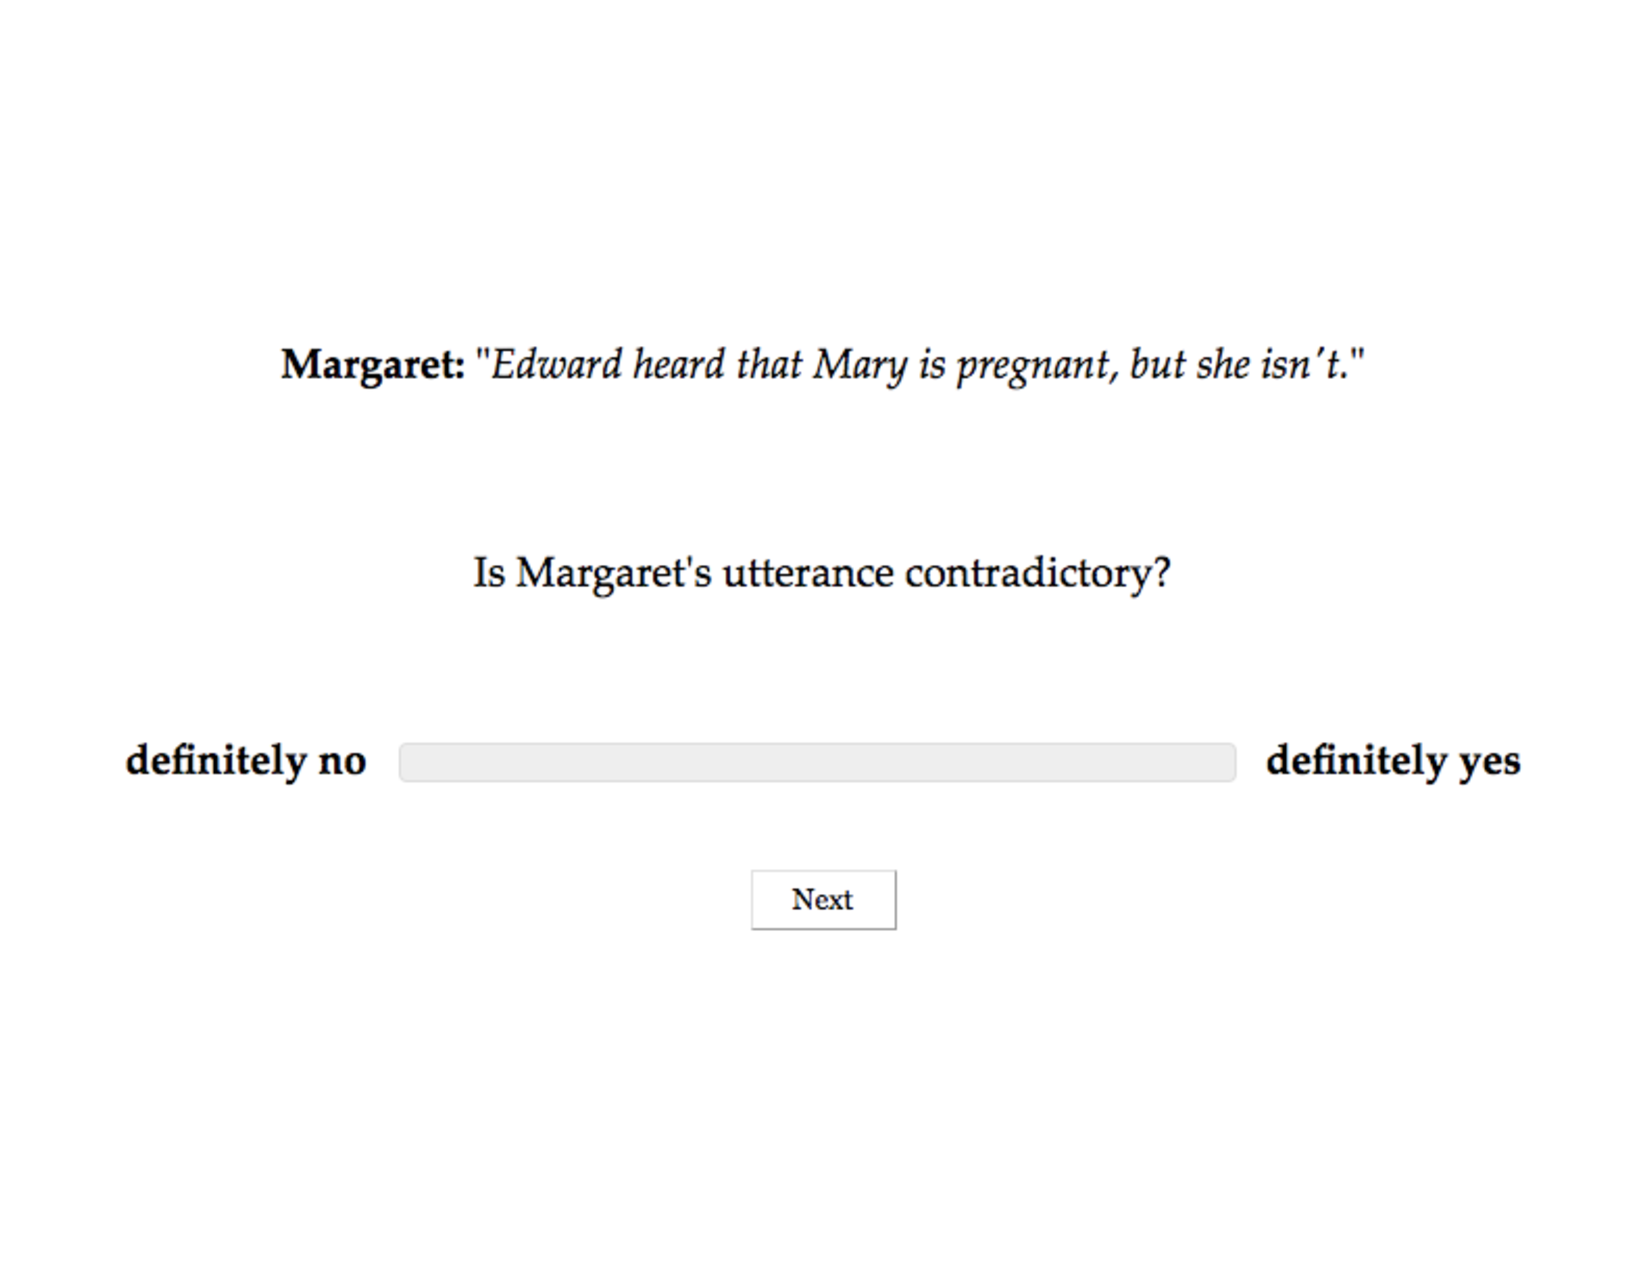
\includegraphics[width=10cm]{figures/contradictory-trial}}
\end{center}
\caption{A sample trial in Experiment 1}\label{f-trial-exp2}
\end{figure}

To familiarize participants with the task, they first completed the two familiarization items in (\ref{train}): participants who rated (\ref{train}a) in the lower half of the scale or (\ref{train}b) in the upper half of the scale were given an explanation for why their answer was wrong. Participants could only advance to the 28 stimuli if they gave the correct rating to the two training stimuli.

\begin{exe}
\ex\label{train}
\begin{xlist}
\ex {\bf Bill:} Drew is aware that Patty lives in Canada, but she doesn't.

\ex {\bf Bob}: Drew thinks that Patty lives in Canada, but she doesn't.
\end{xlist}
\end{exe}

After responding to the 28 stimuli, participants filled out a short, optional survey about their age, their gender, their native language(s) and, if English is their native language, whether they are a speaker of American English (as opposed to, e.g., Australian or Indian English). To encourage them to respond truthfully, participants were told that they would be paid no matter what answers they gave in the survey.

\paragraph{Data exclusion}
Prior to analysis, the data from 19 participants who did not self-identify as native speakers of American English were excluded. For the remaining 281 participants, we inspected their responses to the 8 control stimuli: we expected low responses to the non-contradictory stimuli in (\ref{control-good}) and high responses to the contradictory stimuli in (\ref{control-bad}). The response means of 12 participants were more than 3 standard deviations above the group mean for the non-contradictory control stimuli or below the group mean for the contradictory control stimuli (the group means were .08 and .94, respectively).\footnote{The response mean of one of the non-contradictory control stimuli, (\ref{control-good}a) {\em Zack believes that I'm married, but I'm actually single}, was higher, at .17, than the response means of the remaining three non-contradictory control stimuli (which were .05 or .06). We hypothesize that some participants gave higher responses to this stimulus because the speaker can be taken to contradict Zack's belief.} Closer inspection revealed that these participants' responses to the control stimuli were systematically higher or lower, suggesting that these participants did not attend to the task or interpreted the task differently. The data from these 12 participants were also excluded, leaving data from 269 participants (ages 18-72; median: 36; 128 female, 140 male, 1 other).  

\subsubsection{Results}

The boxplot in Figure \ref{f-veridicality-predicate} shows the contradictoriness ratings by predicate, collapsing over the 20 complement clauses that each predicate was paired with. Predicates whose clausal complement is typically taken to not be an entailment are given in brown, predicates whose clausal complement is typically taken to be an entailment are given in blue, and apparently-entailing predicates are given in black. As expected, stimuli with the 5 non-entailing predicates, namely {\em pretend, suggest, think, hear} and {\em say}, received the lowest contradictoriness ratings. Likewise, the median rating and the mean rating of stimuli with {\em be right} were at and close to ceiling, respectively, in line with the assumption that the content of the clausal complement of this predicate is entailed. However, the median and mean ratings of stimuli with the other entailing predicates were not consistently high and, crucially, many were lower the median and mean ratings of stimuli with apparently-entailing predicates. 

\begin{figure}[h!]
\centering

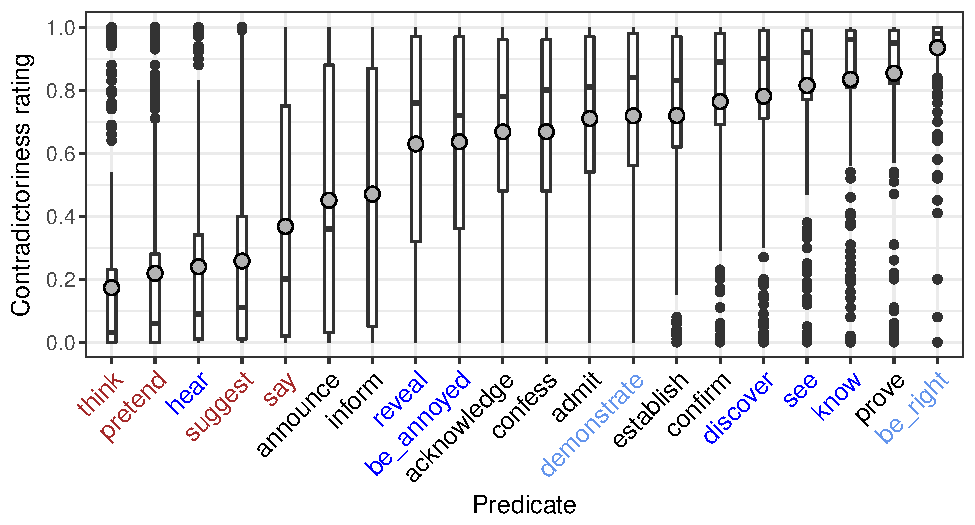
\includegraphics[width=.8\paperwidth]{../results/2-veridicality2/graphs/boxplot-veridicality}

\caption{Boxplot of contradictoriness ratings by predicate, collapsing across complement clauses. Grey dots indicate means and notches indicate medians. Non-entailing predicates are given in brown, entailing predicates in blue, and the remaining predicates are given in black.}
\label{f-veridicality-predicate}
\end{figure}

To determine which predicates differed from one another in the contradictoriness ratings, we conducted post hoc pairwise comparisons using Tukey's method (allowing for by-participant variability), using the \verb|lsmeans| package \citep{tukey} in R \citep{r}. P-values for each pair of predicates are displayed in Table \ref{t-pairwise}. This analysis confirmed that the 5 non-entailing predicates received significantly lower contradictoriness ratings than the 7 entailing predicates, which is in line with the assumption that non-entailing and entailing predicates differ in the status of the content of their clausal complement. The 5 non-entailing predicates also received significantly lower contradictoriness ratings than the 8 apparently-entailing predicates. This finding reflects the observation, made in the literature, that the content of the clausal complement is more likely be taken to follow from utterances of unembedded sentences with apparently-entailing predicates than from utterances of unembedded sentences with non-entailing predicates. 

We also observe, however, that the contradictoriness ratings do not neatly separate entailing from apparently-entailing predicates. For instance, the contradictoriness ratings for stimuli with the entailing predicate {\em know} were indistinguishable from those with the apparently-entailing predicate {\em prove}, as were those with the entailing predicate {\em be annoyed} and the apparently-entailing predicate {\em confess}. 
Crucially, contradictoriness ratings for stimuli with entailing predicates were not, as a whole, higher than for stimuli with apparently-entailing predicates. For instance, stimuli with the entailing predicate {\em reveal} received significantly lower contradictoriness ratings than those with the apparently-entailing predicates {\em demonstrate} and {\em confirm}, and stimuli with the entailing predicates {\em establish} received significantly lower ratings than those with the apparently-entailing predicate {\em prove}. What's more, the contradictoriness diagnostic is suggestive of significant differences between entailing predicates: the contradictoriness ratings for stimuli with {\em reveal} and {\em be annoyed} were significantly lower than those with {\em establish}, which in turn were significantly lower than those with {\em discover, see} and {\em know}, which in turn were significantly lower than those with {\em be right}. Finally, note that stimuli with {\em inform} are statistically indistinguishable from those with the apparently-entailing predicate {\em announce}. As a consequence, the experiment results are inconclusive about whether {\em inform} is an entailing predicate (as maintained in \citealt{schlenker10}) or an apparently-entailing predicate (as maintained in \citealt{anand-hacquard2014}). However, at the very least, the contradictoriness diagnostic does not provide empirical motivation for treating the two predicates differently based on whether they entail the content of the clausal complement.

Overall, then, the contradictoriness diagnostic for entailment does not provide empirical evidence for a categorical distinction between non-entailing and apparently-entailing predicates, on the one hand, and entailing predicates, on the other hand. Rather, the findings of Exp.~1a suggest that the extent to which the content of the clausal complement follows from an utterance of an unembedded sentence is a gradient property. 

\begin{landscape}
\begin{table}[h!]
\centering
\begin{tabular}{l l l l l l l l l l l l l l l l l l l l }
\toprule

 &   \rot{\color{brown}{\em think}\color{black}} & \rot{\color{brown}{\em pretend}\color{black}} & \rot{\color{brown}{\em hear}\color{black}} &  \rot{\color{brown}{\em suggest}\color{black}} &  \rot{\color{brown}{\em say}\color{black}} & \rot{{\em announce}} & \rot{{\em inform}} & \rot{\color{blue}{\em reveal}\color{black}} & \rot{\color{blue}{\em be annoyed}\color{black}} & \rot{{\em confess}} & \rot{{\em acknowledge}} & \rot{{\em admit}} & \rot{\color{blue}{\em establish}\color{black}}  & \rot{{\em demonstrate}}  & \rot{{\em confirm}}  & \rot{\color{blue}{\em discover}\color{black}} & \rot{\color{blue}{\em see}\color{black}}  & \rot{\color{blue}{\em know}\color{black}}  & \rot{{\em prove}}  \\
\midrule
%\color{brown}{\em think}\color{black}		& -- & - & - & - & - & - & - & - & - & - & - & - & - & - & - & - & - & - & - \\
\color{brown}{\em pretend}\color{black}		& n.s. & - & - & - & - & - & - & - & - & - & - & - & - & - & - & - & - & - & - \\
\color{brown}{\em hear}\color{black}			& n.s. & n.s. & - & - & - & - & - & - & - & - & - & - & - & - & - & - & - & - & - \\
\color{brown}{\em suggest}	\color{black}		& * & n.s. & n.s. & - & - & - & - & - & - & - & - & - & - & - & - & - & - & - & - \\
\color{brown}{\em say}\color{black}		& *** & *** & *** & ** & - & - & - & - & - & - & - & - & - & - & - & - & - & - & - \\
\color{black}{\em announce}\color{black}		& *** & *** & *** & *** & * & - & - & - & - & - & - & - & - & - & - & - & - & - & - \\
\color{black}{\em inform}\color{black}		& *** & *** & *** & *** & ** & n.s. & - & - & - & - & - & - & - & - & - & - & - & - & - \\
\color{blue}{\em reveal}\color{black}		& *** & *** & *** & *** & *** & *** & *** & - & - & - & - & - & - & - & - & - & - & - & - \\
\color{blue}{\em be annoyed}\color{black}		& *** & *** & *** & *** & *** & *** & *** & n.s. & - & - & - & - & - & - & - & - & - & - & - \\
\color{black}{\em confess}\color{black}		& *** & *** & *** & *** & *** & *** & *** & n.s. & n.s. & - & - & - & - & - & - & - & - & - & - \\
\color{black}{\em acknowledge}\color{black}	& *** & *** & *** & *** & *** & *** & *** & n.s. & n.s. & n.s. & - & - & - & - & - & - & - & - & - \\
\color{black}{\em admit}\color{black}			& *** & *** & *** & *** & *** & *** & *** & * & . & n.s. & n.s. & - & - & - & - & - & - & - & - \\
\color{blue}{\em establish}\color{black}		& *** & *** & *** & *** & *** & *** & *** & ** & * & n.s. & n.s. &  n.s. & - & - & - & - & - & - & - \\
\color{black}{\em demonstrate}\color{black}	& *** & *** & *** & *** & *** & *** & *** & ** & * & n.s. & n.s. & n.s. & n.s. & - & - & - & - & - & - \\
\color{black}{\em confirm}\color{black}		& *** & *** & *** & *** & *** & *** & *** & *** & *** & ** & ** & n.s. & n.s. & n.s. & - & - & - & - & - \\
\color{blue}{\em discover}\color{black}		& *** & *** & *** & *** & *** & *** & *** & *** & *** & ** & ** & n.s. & n.s. & n.s. & n.s. & - & - & - & - \\
\color{blue}{\em see}\color{black}			& *** & *** & *** & *** & *** & *** & *** & *** & *** & *** & *** & ** & ** & ** & n.s. & n.s. & - & - & - \\
\color{blue}{\em know}\color{black}			& *** & *** & *** & *** & *** & *** & *** & *** & *** & *** & *** & *** & *** & *** & n.s. & n.s. & n.s. & - & - \\
\color{black}{\em prove}\color{black}			& *** & *** & *** & *** & *** & *** & *** & *** & *** & *** & *** & *** & *** & *** & ** & n.s. & n.s. & n.s. & -  \\
\color{blue}{\em be right}\color{black}		& *** & *** & *** & *** & *** & *** & *** & *** & ***  & ***  & *** & *** & *** & *** & *** & *** & *** & ** & *  \\

\bottomrule
\end{tabular}
\caption{P-values associated with pairwise comparison of contradictoriness ratings of predicates using Tukey's method. `***' indicates significance at .0001, `**' at .01, `*' at .05, `.' marginal significance at .1, and `n.s' indicates no significant difference in means. Non-entailing predicates are given in brown, entailing predicates are given in blue, and apparently-entailing predicates are given in black.}\label{t-pairwise}
\end{table}
\end{landscape}

In Figure \ref{f-veridicality-predicate}, the large box sizes and long whisker lengths for many of the predicates was already suggestive of by-participant variation in the extent to which stimuli with such predicates were assessed to be contradictory. By-participant variation in contradictoriness ratings is also revealed in the top panel of Figure \ref{f-contradict-participant}, which gives participants' mean contradictoriness ratings over all 20 predicates. The bottom panel of Figure \ref{f-contradict-participant} shows that there is also by-participant variability in participants' mean contradictoriness ratings over the 7 entailing predicates.

\begin{figure}[h!]
\centering

\subfloat[][Mean contradictoriness ratings over all predicates.]{ 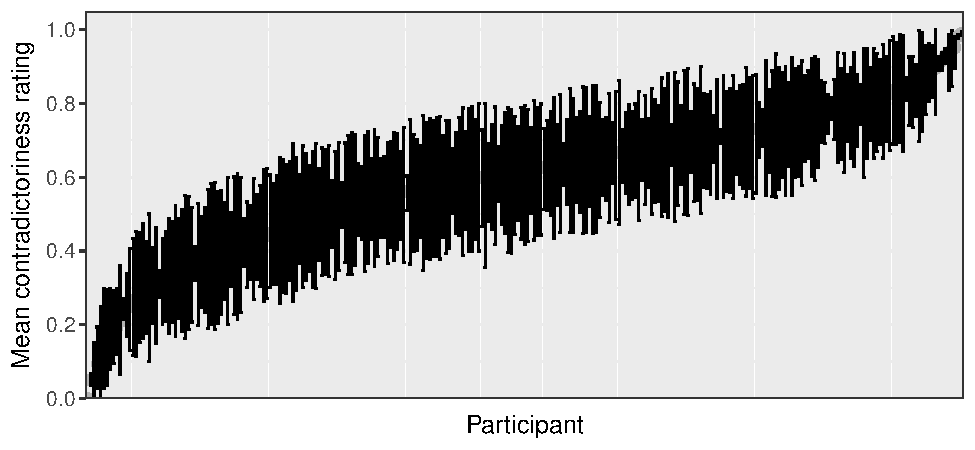
\includegraphics[width=.8\paperwidth]{../results/2-veridicality2/graphs/veridicality-subjmeans}
}

\subfloat[][Mean contradictoriness ratings over entailing predicates.]{ 
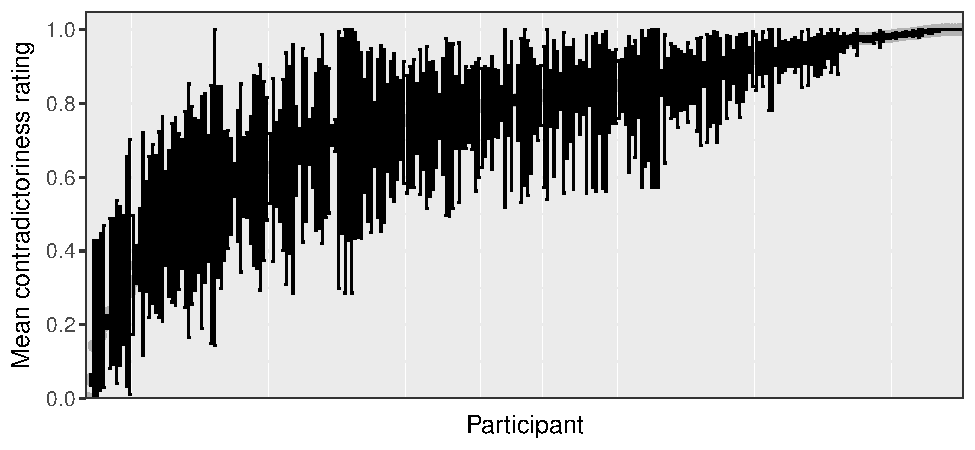
\includegraphics[width=.8\paperwidth]{../results/2-veridicality2/graphs/veridicality-entailing-subjmeans}
	}

\caption{Mean contradictoriness ratings by participant, collapsing across predicates and complement clauses. Grey dots indicate means and error bars indicate bootstrapped 95\% confidence intervals.}
\label{f-contradict-participant}
\end{figure}

\subsubsection{Discussion}

\begin{itemize}

\item Contradictoriness diagnostic for entailment distinguishes non-entailing predicates from entailing predicates but does not distinguish apparently-entailing from entailing predicates

\item The diagnostic doesn't seem to diagnose entailment but rather the extent to which the speaker has signalled their commitment to the truth of the content of the complement.

In other words: because of the way the diagnostic is set up, it provides insight into the extent to which the inference that the speaker is committed to the truth of p is cancelable/defeasible (and can therefore reveal something about how the inference arose, which in turn reveals something about whether it survives embedding). 

\begin{itemize}

\item {\em be right} presupposes that the subject believes p and asserts that the speaker is committed to the truth of p; speaker commitment does not survive embedding

\item {\em prove} asserts that the subject (logically) deduced p; by using {\em prove} and not saying anything to the contrary, the speaker implies that they believe this (logical) deduction to be valid and, therefore, that they are committed to the truth of p; embedding removes assertion that subject deduced p, hence implication doesn't arise

\item {\em know} asserts that the subject is committed to the truth of p

\item {\em see} asserts that the subject is committed to p, given their access to direct evidence for p (DIR(p)); by using {\em see}, the speaker is taken to be committed to DIR(p) and therefore to the truth of p; embedding removes the assertion but leaves open the possibility that there is direct/conjectural evidence for p; speaker commitment can remain

{\bf Why are {\em see} and {\em prove} alike wrt entailment, but not wrt projection? Why are {\em hear} and {\em see} different wrt entailment, but alike wrt projection?}

know: entail+, proj+		sp commitment is not tied to subject knowing
\\ see: entail+, proj+			sp commitment is not tied to subject having direct evid
\\ hear: entail-, proj+		subj indirect evidence not enough for sp commitment
\\ prove: entail+, proj-		speaker commitment is tied to proof by subject
\\ be-right: entail+, proj-
\\ think: entail-, proj-

speaker commitment in unembedded case may arise in different ways, which has implications for speaker commitment under operator

sp commitment asserted (be right): doesn't survive

sp commitment tied to subject action (prove): doesn't survive
\\ with discover, sp commitment is not tied to subject's action of discovering; rather the fact that p is independent of subject's discovery

sp commitment tied to backgrounded evidence (see): survives

no sp commitment w/ hear: there is (only) reportative evidence for p; under operator, 

\item {\em discover} asserts that the subject went from not knowing p to knowing p; by using {\em discover} and not saying anything to the contrary, the speaker implies that they are committed to p; embedding removes subject's change from not-p to p, but leaves open the possibility that p is the case; speaker commitment can remain

\item {\em announce, inform, say} convey that the subject uttered a clause denoting p; depending on p and the subject's authority, the speaker may be taken to be committed to the truth of p

\end{itemize}

\item Possible that participants interpreted ``contradictory'' differently especially for the verbs of saying

\end{itemize}

\subsection{Experiment 1b: How likely is {\em B} given {\em A}?}

This experiment explored whether the content of the clausal complement of 20 clause-embedding English predicates is entailed. Specifically, this experiment implemented the diagnostic for entailment from \citealt{ccmg90} according to which {\em A} entails {\em B} if and only if {\em B} follows from {\em A}. Gradient inference ratings were collected.

\subsubsection{Methods}\label{s-methods2}

\paragraph{Participants} 300 participants with U.S.\ IP addresses and at least 99\% of previous HITs approved were recruited on Amazon's Mechanical Turk platform (ages: XX-XX, median: XX; XX female, XX male, X other). They were paid 75 cents for participating in the experiment.

\paragraph{Materials} Whether the content of the clausal complement was entailed was tested for the same 20 clause-embedding predicates as in Exp.~1. Each predicate was paired with each of the 20 event-describing sentences from section \ref{s-norming-prior} and a proper name subject, for a total of 400 sentences.\footnote{Eventive predicates, like {\em discover} and {\em hear}, were realized in the past tense and stative predicates, like {\em know} and {\em be annoyed}, were realized in the present tense. The indirect object of {\em inform} was realized by the proper name {\em Sam}.} The 400 target stimuli consisted of one of these 400 sentences, as shown in the sample stimuli in (\ref{stims2}). The speaker of the target stimuli was realized by a (bold-faced) proper name. The proper names that realized the speakers, the subjects of the 20 predicates or that occurred in the complement clauses were all unique. 

\begin{exe}
\ex\label{stims2}
\begin{xlist}
\ex Fact: Melissa knows that Danny ate the last cupcake.
\\ How likely is it that Danny ate the last cupcake?
\ex Fact: Jerry pretended that Emma studied on Saturday morning.
\\ How likely is it that Emma studied on Saturday morning?
\end{xlist}
\end{exe}

The experiment also included eight control stimuli, which were used to assess whether participants were attending to the task and to allow participants to use the full response scale. The four control stimuli in (\ref{control-good}) were hypothesized to be non-contradictory, and the four control stimuli in (\ref{control-bad}) were hypothesized to be contradictory.

\begin{exe}
\ex\label{control-good2}
\begin{xlist}
\ex Zack believes that I'm married, but I'm actually single.
\ex Tara wants me to cook for her and I'm a terrific cook.
\ex Frederick is both smarter and taller than I am.
\ex Vanessa is really good at math, but I'm not.
\end{xlist}
\ex\label{control-bad2}
\begin{xlist}
\ex Dana has never smoked in her life and she stopped smoking recently.
\ex Hendrick's car is completely red and his car is not red.
\ex Madison laughed loudly and she didn't laugh.
\ex Sebastian lives in the USA and has never been to the USA.
\end{xlist}
\end{exe}

Each participant saw a random set of 28 stimuli: each set contained one stimulus for each of the 20 predicates (each with a unique complement clause) and the same 8 control stimuli. Trial order was randomized.


\paragraph{Procedure} Participants were told that they would read utterances made by a speaker and were asked to assess whether the speaker's utterance is contradictory. On each trial, participants read the speaker's utterance and then gave their response on a slider marked `definitely no' at one end (coded as 0) and `definitely yes' at the other (coded as 1), as shown in Figure \ref{f-trial-exp3}.

\begin{figure}[h!]
\begin{center}
\fbox{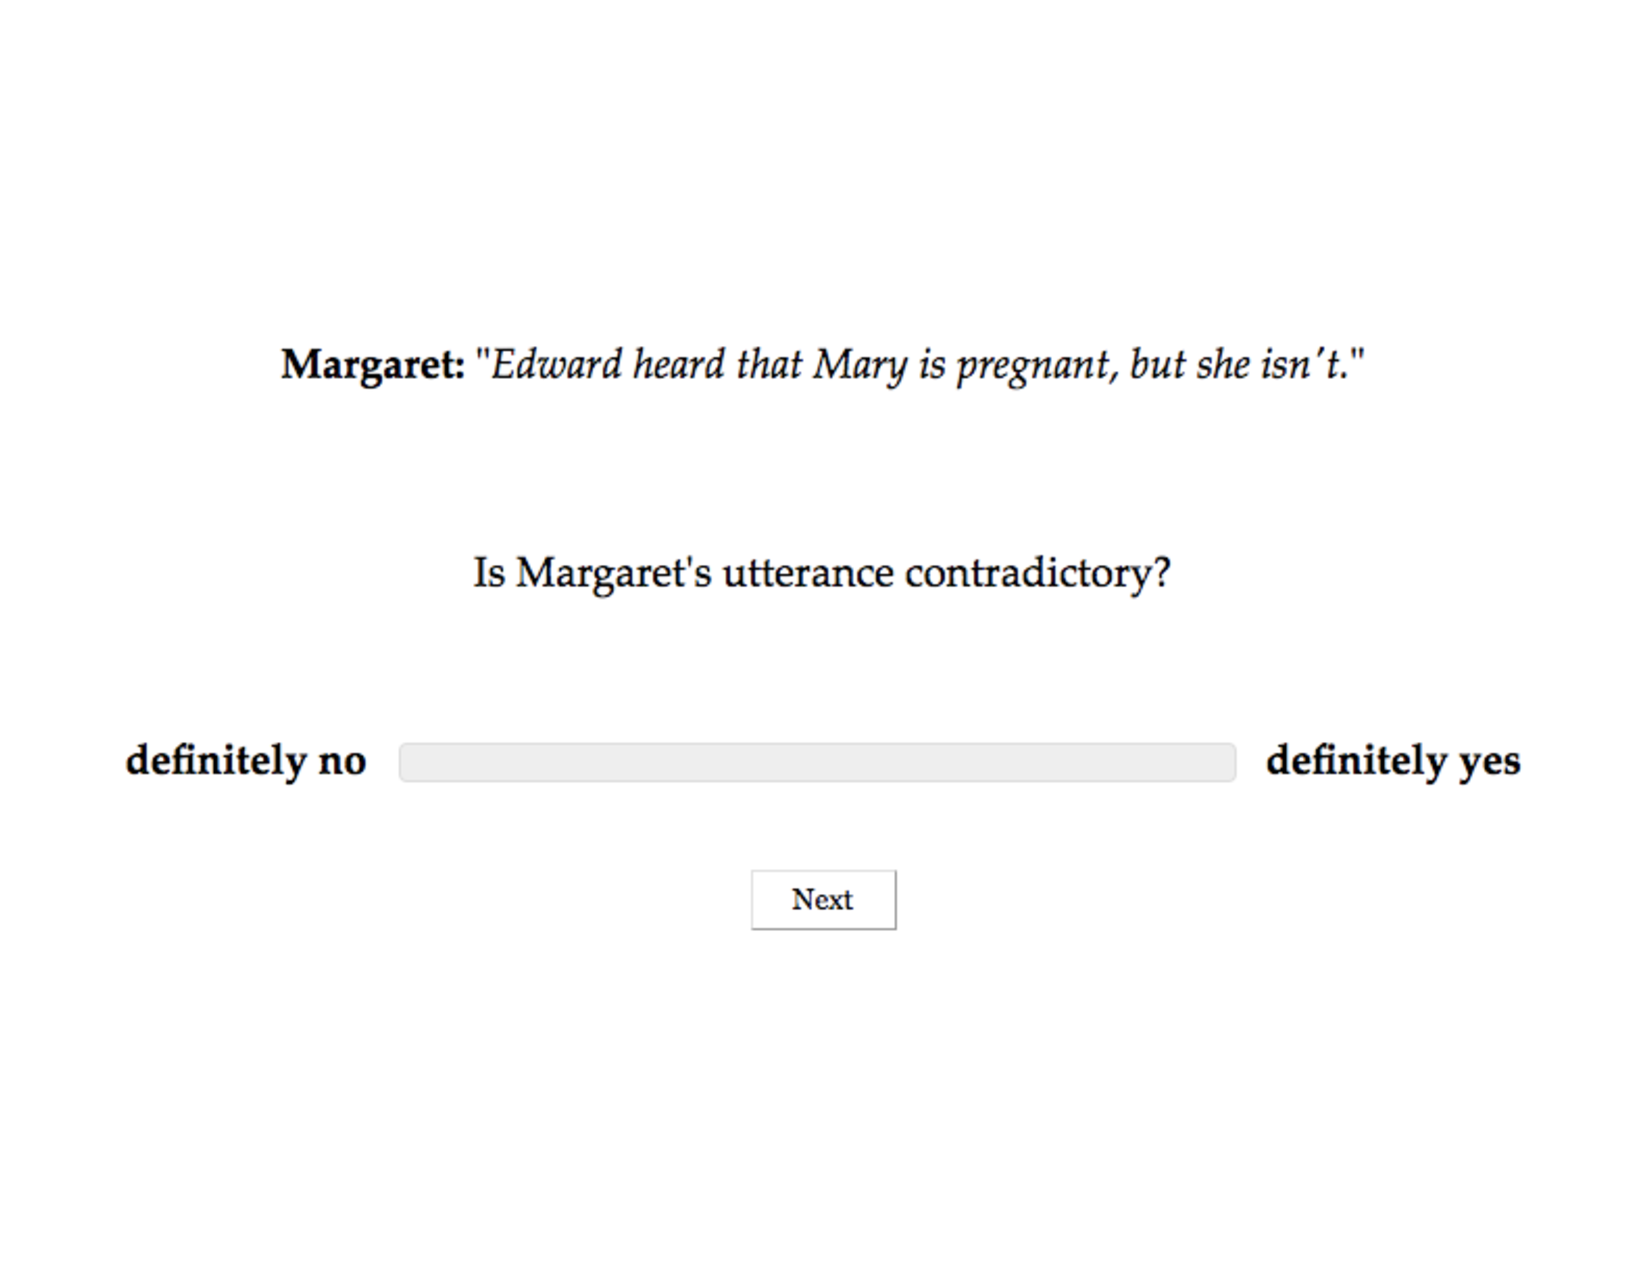
\includegraphics[width=10cm]{figures/contradictory-trial}}
\end{center}
\caption{A sample trial in Experiment 2}\label{f-trial-exp3}
\end{figure}

To familiarize participants with the task, they first completed the two familiarization items in (\ref{train2}): participants who rated (\ref{train2}a) in the lower half of the scale or (\ref{train2}b) in the upper half of the scale were given an explanation for why their answer was wrong. Participants could only advance to the 28 stimuli if they gave the correct rating to the two training stimuli.

\begin{exe}
\ex\label{train2}
\begin{xlist}
\ex {\bf Bill:} Drew is aware that Patty lives in Canada, but she doesn't.

\ex {\bf Bob}: Drew thinks that Patty lives in Canada, but she doesn't.
\end{xlist}
\end{exe}

After responding to the 28 stimuli, participants filled out a short, optional survey about their age, their gender, their native language(s) and, if English is their native language, whether they are a speaker of American English (as opposed to, e.g., Australian or Indian English). To encourage them to respond truthfully, participants were told that they would be paid no matter what answers they gave in the survey.

\paragraph{Data exclusion}
Prior to analysis, the data from XX participants who did not self-identify as native speakers of American English were excluded. For the remaining XXX participants, we inspected their responses to the XX control stimuli: we expected low responses to the non-contradictory stimuli in (\ref{control-good2}) and high responses to the contradictory stimuli in (\ref{control-bad2}). The response means of XX participants were more than 3 standard deviations above the group mean for the non-contradictory control stimuli or below the group mean for the contradictory control stimuli (the group means were .08 and .94, respectively). Closer inspection revealed that these participants' responses to the control stimuli were systematically higher or lower, suggesting that these participants did not attend to the task or interpreted the task differently. The data from these XX participants were also excluded, leaving data from XX participants (ages XX-XX; median: XX; XX female, XX male, XX other).  

\subsubsection{Results}

The boxplot in Figure \ref{f-veridicality-predicate2} shows the contradictoriness ratings by predicate, collapsing over the 20 complement clauses that each predicate was paired with. Predicates whose clausal complement is typically taken to not be an entailment are given in brown, predicates whose clausal complement is typically taken to be an entailment are given in blue, and apparently-entailing predicates are given in black. 

\begin{figure}[h!]
\centering

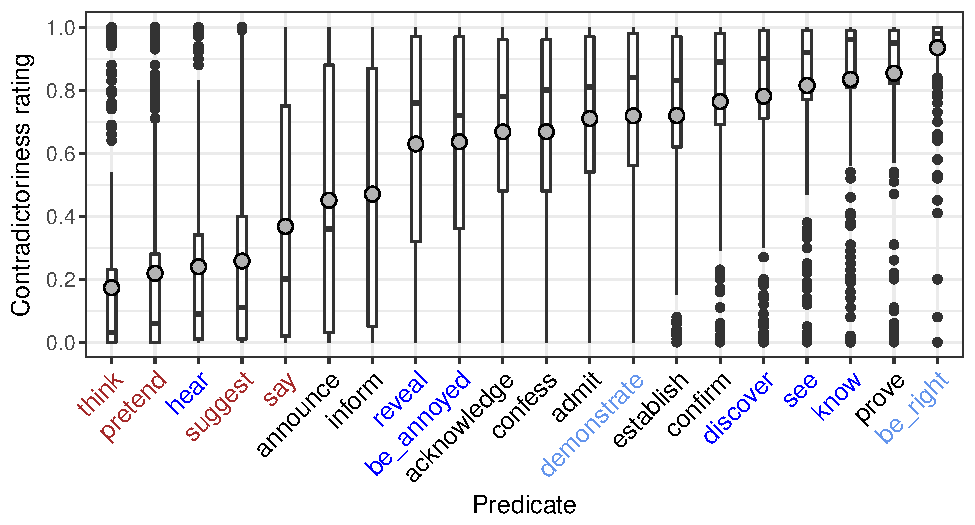
\includegraphics[width=.8\paperwidth]{../results/2-veridicality2/graphs/boxplot-veridicality}

\caption{Boxplot of XXX ratings by predicate, collapsing across complement clauses. Grey dots indicate means and notches indicate medians. Non-entailing predicates are given in brown, entailing predicates in blue, and the remaining predicates are given in black.}
\label{f-veridicality-predicate2}
\end{figure}


\begin{landscape}
\begin{table}[h!]
\centering
\begin{tabular}{l l l l l l l l l l l l l l l l l l l l }
\toprule

 &   \rot{\color{brown}{\em think}\color{black}} & \rot{\color{brown}{\em pretend}\color{black}} & \rot{\color{brown}{\em hear}\color{black}} &  \rot{\color{brown}{\em suggest}\color{black}} &  \rot{\color{brown}{\em say}\color{black}} & \rot{{\em announce}} & \rot{{\em inform}} & \rot{\color{blue}{\em reveal}\color{black}} & \rot{\color{blue}{\em be annoyed}\color{black}} & \rot{{\em confess}} & \rot{{\em acknowledge}} & \rot{{\em admit}} & \rot{\color{blue}{\em establish}\color{black}}  & \rot{{\em demonstrate}}  & \rot{{\em confirm}}  & \rot{\color{blue}{\em discover}\color{black}} & \rot{\color{blue}{\em see}\color{black}}  & \rot{\color{blue}{\em know}\color{black}}  & \rot{{\em prove}}  \\
\midrule
%\color{brown}{\em think}\color{black}		& -- & - & - & - & - & - & - & - & - & - & - & - & - & - & - & - & - & - & - \\
\color{brown}{\em pretend}\color{black}		& n.s. & - & - & - & - & - & - & - & - & - & - & - & - & - & - & - & - & - & - \\
\color{brown}{\em hear}\color{black}			& n.s. & n.s. & - & - & - & - & - & - & - & - & - & - & - & - & - & - & - & - & - \\
\color{brown}{\em suggest}	\color{black}		& * & n.s. & n.s. & - & - & - & - & - & - & - & - & - & - & - & - & - & - & - & - \\
\color{brown}{\em say}\color{black}		& *** & *** & *** & ** & - & - & - & - & - & - & - & - & - & - & - & - & - & - & - \\
\color{black}{\em announce}\color{black}		& *** & *** & *** & *** & * & - & - & - & - & - & - & - & - & - & - & - & - & - & - \\
\color{black}{\em inform}\color{black}		& *** & *** & *** & *** & ** & n.s. & - & - & - & - & - & - & - & - & - & - & - & - & - \\
\color{blue}{\em reveal}\color{black}		& *** & *** & *** & *** & *** & *** & *** & - & - & - & - & - & - & - & - & - & - & - & - \\
\color{blue}{\em be annoyed}\color{black}		& *** & *** & *** & *** & *** & *** & *** & n.s. & - & - & - & - & - & - & - & - & - & - & - \\
\color{black}{\em confess}\color{black}		& *** & *** & *** & *** & *** & *** & *** & n.s. & n.s. & - & - & - & - & - & - & - & - & - & - \\
\color{black}{\em acknowledge}\color{black}	& *** & *** & *** & *** & *** & *** & *** & n.s. & n.s. & n.s. & - & - & - & - & - & - & - & - & - \\
\color{black}{\em admit}\color{black}			& *** & *** & *** & *** & *** & *** & *** & * & . & n.s. & n.s. & - & - & - & - & - & - & - & - \\
\color{blue}{\em establish}\color{black}		& *** & *** & *** & *** & *** & *** & *** & ** & * & n.s. & n.s. &  n.s. & - & - & - & - & - & - & - \\
\color{black}{\em demonstrate}\color{black}	& *** & *** & *** & *** & *** & *** & *** & ** & * & n.s. & n.s. & n.s. & n.s. & - & - & - & - & - & - \\
\color{black}{\em confirm}\color{black}		& *** & *** & *** & *** & *** & *** & *** & *** & *** & ** & ** & n.s. & n.s. & n.s. & - & - & - & - & - \\
\color{blue}{\em discover}\color{black}		& *** & *** & *** & *** & *** & *** & *** & *** & *** & ** & ** & n.s. & n.s. & n.s. & n.s. & - & - & - & - \\
\color{blue}{\em see}\color{black}			& *** & *** & *** & *** & *** & *** & *** & *** & *** & *** & *** & ** & ** & ** & n.s. & n.s. & - & - & - \\
\color{blue}{\em know}\color{black}			& *** & *** & *** & *** & *** & *** & *** & *** & *** & *** & *** & *** & *** & *** & n.s. & n.s. & n.s. & - & - \\
\color{black}{\em prove}\color{black}			& *** & *** & *** & *** & *** & *** & *** & *** & *** & *** & *** & *** & *** & *** & ** & n.s. & n.s. & n.s. & -  \\
\color{blue}{\em be right}\color{black}		& *** & *** & *** & *** & *** & *** & *** & *** & ***  & ***  & *** & *** & *** & *** & *** & *** & *** & ** & *  \\

\bottomrule
\end{tabular}
\caption{P-values associated with pairwise comparison of XXX ratings of predicates using Tukey's method. `***' indicates significance at .0001, `**' at .01, `*' at .05, `.' marginal significance at .1, and `n.s' indicates no significant difference in means. Non-entailing predicates are given in brown, entailing predicates are given in blue, and apparently-entailing predicates are given in black.}\label{t-pairwise2}
\end{table}
\end{landscape}

In Figure \ref{f-veridicality-predicate2}, the large box sizes and long whisker lengths for many of the predicates was already suggestive of by-participant variation in the extent to which stimuli with such predicates were assessed to be contradictory. By-participant variation in contradictoriness ratings is also revealed in the top panel of Figure \ref{f-contradict-participant2}, which gives participants' mean contradictoriness ratings over all 20 predicates. The bottom panel of Figure \ref{f-contradict-participant2} shows that there is also by-participant variability in participants' mean contradictoriness ratings over the 7 entailing predicates.

\begin{figure}[h!]
\centering

\subfloat[][Mean contradictoriness ratings over all predicates.]{ 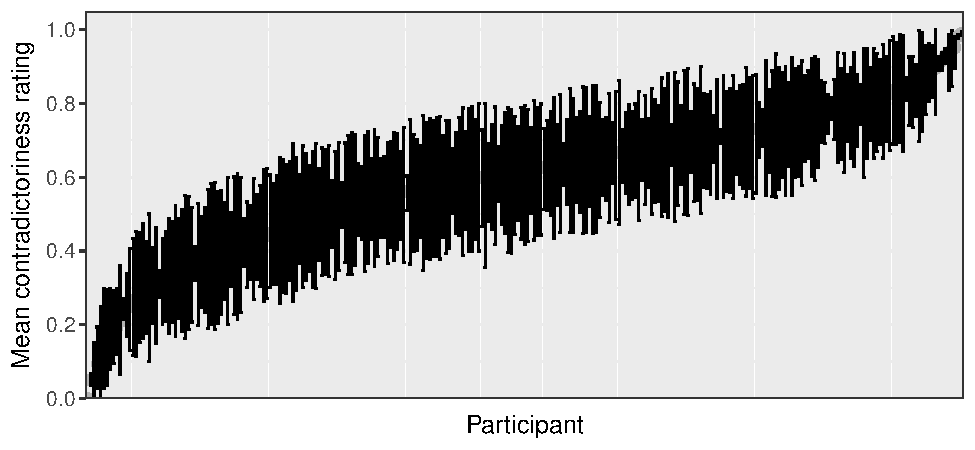
\includegraphics[width=.8\paperwidth]{../results/2-veridicality2/graphs/veridicality-subjmeans}
}

\subfloat[][Mean contradictoriness ratings over entailing predicates.]{ 
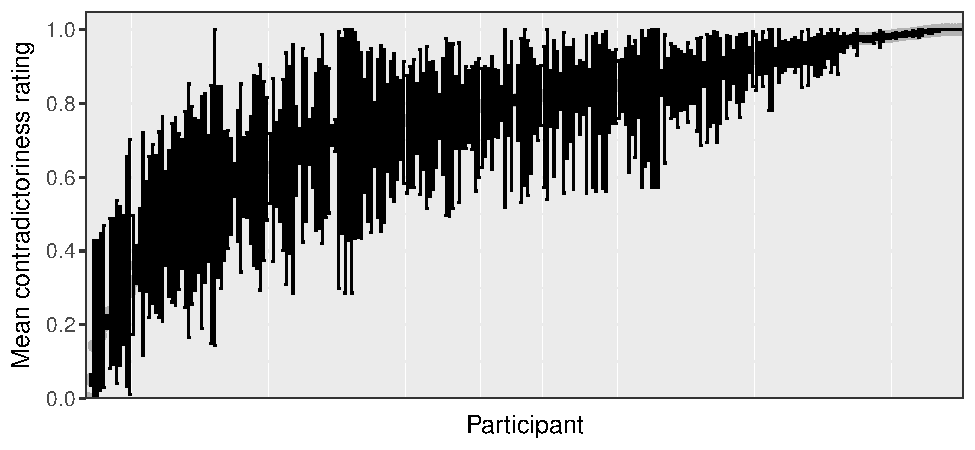
\includegraphics[width=.8\paperwidth]{../results/2-veridicality2/graphs/veridicality-entailing-subjmeans}
	}

\caption{Mean contradictoriness ratings by participant, collapsing across predicates and complement clauses. Grey dots indicate means and error bars indicate bootstrapped 95\% confidence intervals.}
\label{f-contradict-participant2}
\end{figure}

\subsubsection{Discussion}

\begin{itemize}

\item 

\end{itemize}

\subsection{Interim summary}

\section{Experiment 2: Projectivity}

This experiment explored the influence of the clause-embedding predicate and of the prior probability of the event described by the embedded clause on the projectivity of the contents of clausal complements of the 20 predicates under investigation. Gradient projectivity ratings were collected.

\subsection{Methods}

\paragraph{Participants} 300 participants with U.S.\ IP addresses and at least 99\% of previous HITs approved were recruited on Amazon's Mechanical Turk platform (ages: 21-72, median: 36; 145 female, 154 male). They were paid 85 cents for participating in the experiment.

\paragraph{Materials} 400 polar questions were formed by combining the 20 predicates with a proper name subject and the 20 event-describing clauses from the experiments in section \ref{s-entailment}. As discussed in the introduction, 6 of the 20 predicates are typically taken to be factive ({\em be annoyed, know, discover, reveal, see, hear}), 7 are typically taken to be non-factive ({\em be right, pretend, think, suggest, say, prove, demonstrate}), and the remaining 7 predicates have been suggested to be ``part-time triggers'' or to give rise to the ``illusion of factivity'' ({\em establish,  confess, announce, acknowledge, admit, confirm, inform}).\footnote{As in the experiments in section \ref{s-entailment}, eventive predicates were realized in the past tense and stative predicates were realized in the present tense. The indirect object of {\em inform} was realized by the proper name {\em Sam}.} For each of the 20 events described by the clausal complements of the predicates, we identified a fact that made the event more likely and a fact that made the event less likely. (The norming study is described in Appendix \ref{s-norming}.) The 800 target stimuli consisted of a polar question uttered by a speaker who was identified by a proper name and either the fact that made the event described by the complement clause more likely or the fact that made the event less likely. In the two sample stimuli in (\ref{stim-project}), the predicate {\em discover} is paired with a clausal complement that describes the event of Julian dancing salsa. This event has a higher prior probability given the fact in (\ref{stim-project}a) than given the fact in (\ref{stim-project}b). As shown, the speaker of the target stimuli was realized by a (bold-faced) proper name. The proper names that realized the speakers, the subjects of the 20 predicates or that occurred in the complement clauses were all unique. 

\begin{exe}
\ex\label{stim-project} 
\begin{xlist}
\ex {\bf Fact (which Carol knows):} Julian is German.  \\ 
{\bf Carol:} Did Sandra discover that Julian dances salsa?

\ex {\bf Fact (which Paul knows):} Julian is Cuban.  \\ 
{\bf Paul:} Did Sandra discover that Julian dances salsa?
\end{xlist}
\end{exe}

The experiment also included six control stimuli, which consisted of a speaker's utterance of a polar question and a fact about the world that was hypothesized to not affect the prior probability of the event described by the polar question. A sample control stimulus is shown in (\ref{control}); the remaining stimuli can be found in Appendix \ref{a-exp2-control}. The six control stimuli were included to assess whether participants were attending to the task and to allow participants to use the full response scale. 

\begin{exe}
\ex\label{control}
{\bf Fact (which Karen knows):} Zack is a member of the golf club.
\\ {\bf Karen:} Is Zack coming to the meeting tomorrow?
\end{exe}


Each participant saw a random set of 28 stimuli: each set contained one stimulus for each of the 20 predicates (each with a unique complement clause) and the same 8 control stimuli. Trial order was randomized.




\paragraph{Procedure} Participants were told to imagine that they are at a party and that, on walking into the kitchen, they overhear somebody ask somebody else a question. They were also told to consider the fact that was presented with the speaker's question. Participants were asked to identify whether the speaker was certain of the content of the clausal complement. They gave the response on a slider marked `no' at one end (coded as 0) and `yes' at the other (coded as 1), as shown in Figure \ref{f-trial-exp3}.

\begin{figure}[h!]
\begin{center}
\fbox{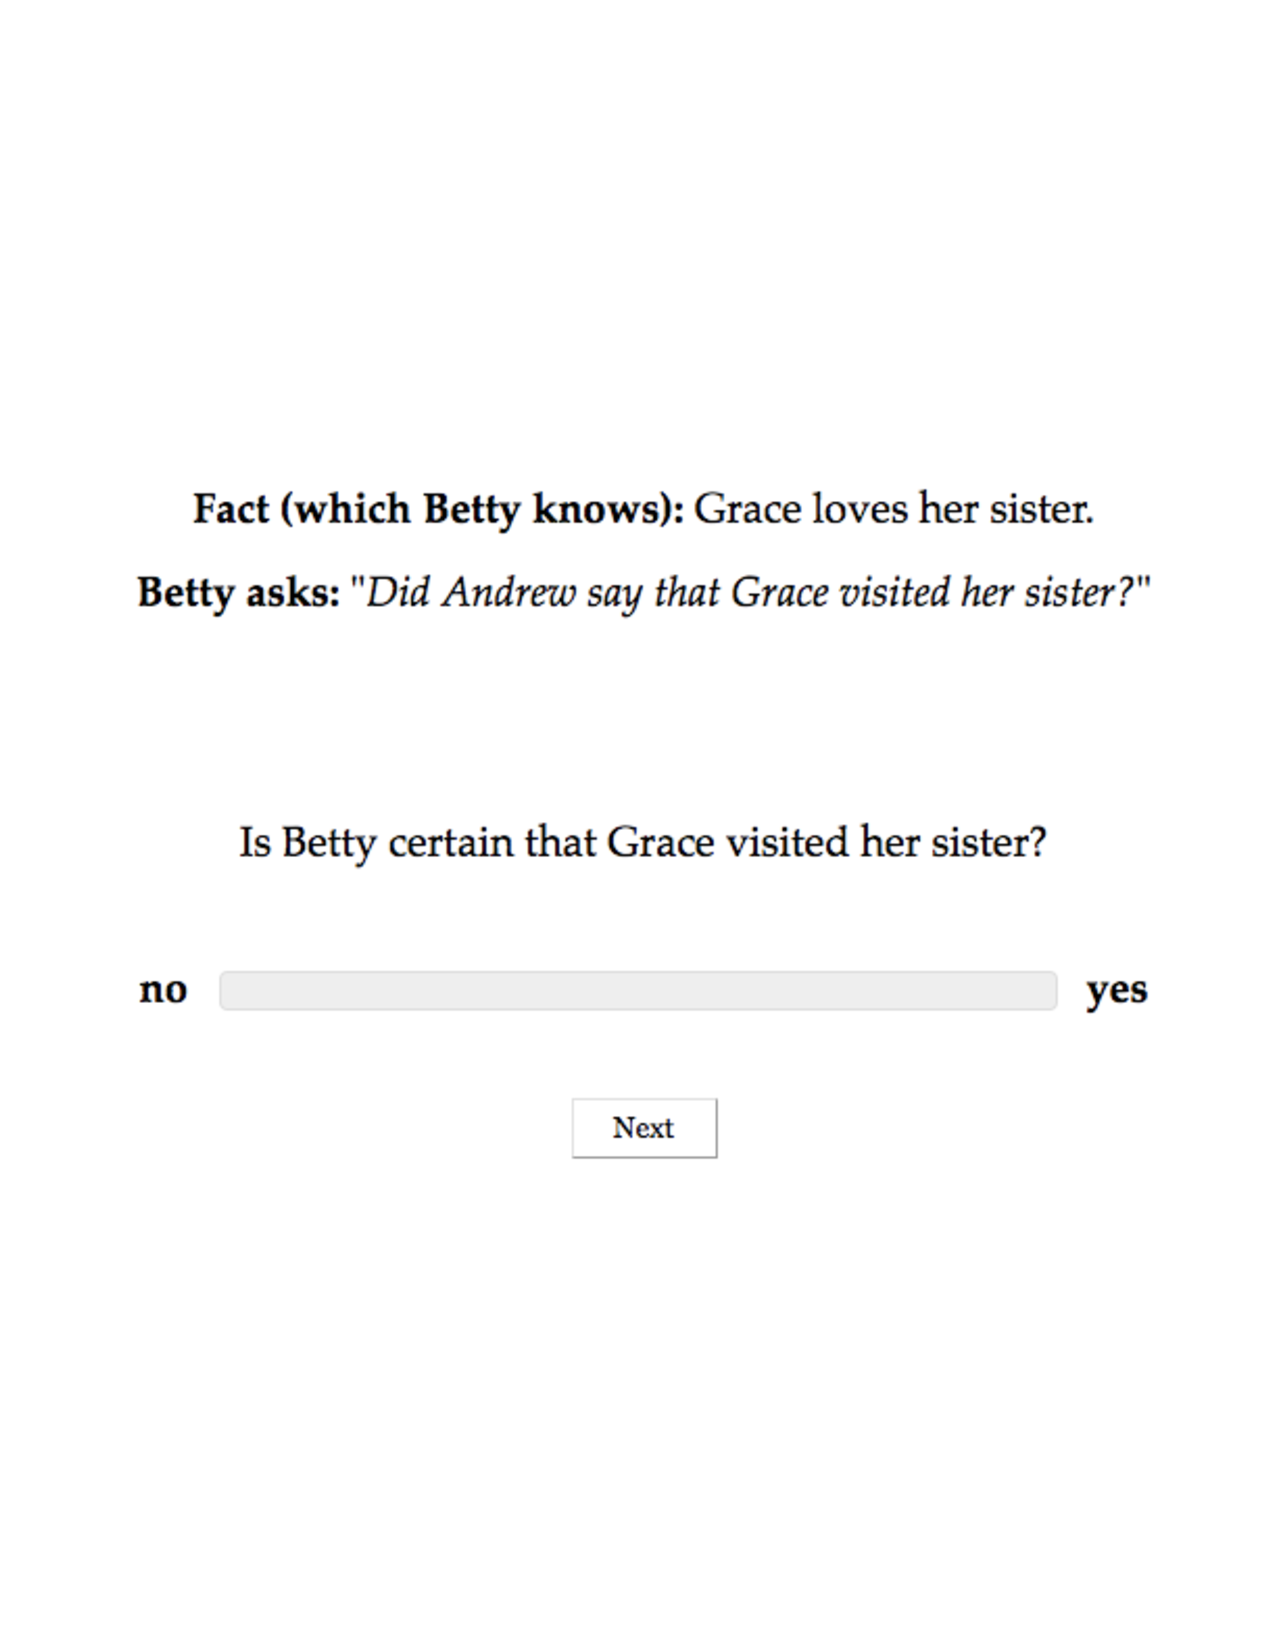
\includegraphics[width=10cm]{figures/proj-trial}}
\end{center}
\caption{A sample trial in Experiment 2}\label{f-trial-exp3}
\end{figure}

After completing the experiment, participants filled out a short, optional survey about their age, their gender, their native language(s) and, if English is their native language, whether they are a speaker of American English (as opposed to, e.g., Australian or Indian English). To encourage them to respond truthfully, participants were told that they would be paid no matter what answers they gave in the survey.

\paragraph{Data exclusion}
Prior to analysis, the data from 23 participants who did not self-identify as native speakers of American English were excluded. For the remaining 277 participants, we inspected their responses to the 6 control stimuli, for which we expected low responses because the main clause content is not expected to project from these questions. The response means of 25 participants were more than 1.5 standard deviations above the group mean of .21 for the control polar question stimuli. Closer inspection revealed that these participants' responses to the control stimuli were systematically higher or lower, suggesting that these participants did not attend to the task or interpreted the task differently. The data from these 25 participants were also excluded, leaving data from 252 participants (ages 21-72; median: 37; 124 female, 128 male).


\subsection{Results}

Mean certainty ratings by predicate and by fact type are shown in Fig.~\ref{f-projectivity}. Overall, mean certainty ratings are higher for for events with a higher prior probability than for events with a lower prior probability. We also observe by-predicate variability in mean certainty ratings: for instance, the content of the clausal complement of {\em pretend} had the lowest mean certainty rating (low prior: .09; high prior: .3) and that of {\em be annoyed} had the highest mean certainty rating (low prior: .55; high prior: .73). These findings suggest that participants considered both the lexical meaning of the predicate and the the prior probability of the event described by the complement clause in identifying whether the speaker was committed to the content of the clausal complement.

\begin{figure}[h!]
\centering

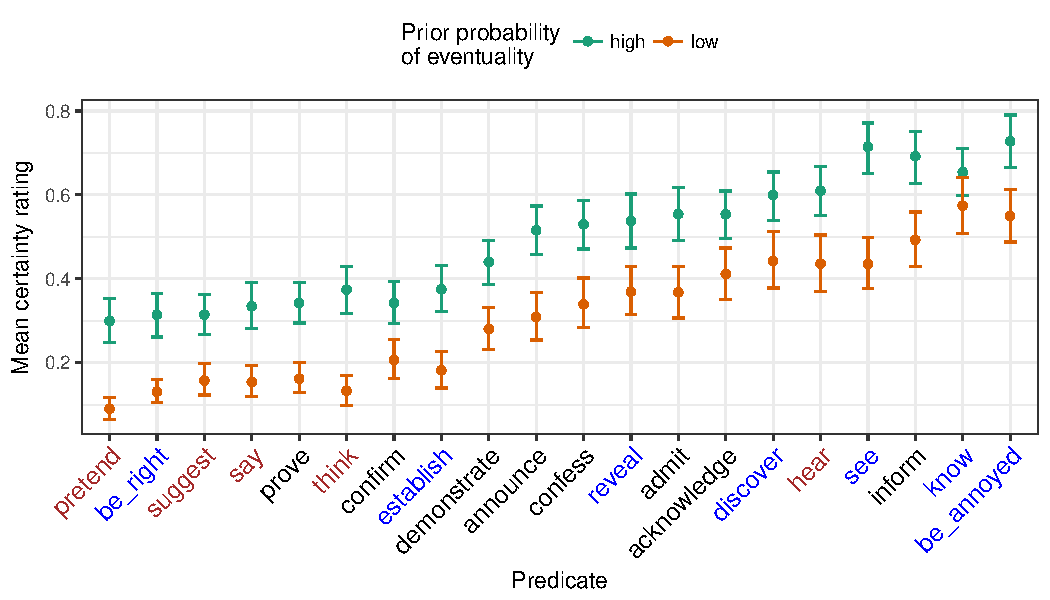
\includegraphics[width=.8\paperwidth]{../results/3-projectivity/graphs/means-projectivity-by-predicate-and-facttype}

\caption{Mean certainty ratings by predicate and fact type, collapsing across complements. Error bars indicate 95\% confidence intervals. Non-entailing predicates are given in brown, entailing predicates are given in blue, and apparently-entailing predicates are given in black.}
\label{f-projectivity}
\end{figure}

The qualitative observation about the influence of the prior probability of events on projectivity was borne out statistically. We conducted a mixed-effects linear regression predicting certainty rating from fixed effects of the mean prior probability of events (norming study), the mean contradictoriness rating of the predicates (Exp.~1a), and their interaction. The model included the maximal random effects structure justified by the data and the theoretical assumptions: random by-participant intercepts (capturing differences in projectivity between participants), random by-content intercepts (capturing differences in projectivity between contents of clausal complements), random by-predicate intercepts (capturing differences in projectivity between predicates), random by-fact intercepts (capturing differences in projectivity between the facts) and random slopes for prior event probability by participant, content and predicate (capturing that the effect of prior event probability may vary across participants, contents, and predicates). {\bf WHAT SENSE DOES PRIOR EVENT PROB SLOPE MAKE FOR CONTENT?} The analysis was conducted on target  trials only (5,040 data points) because we were specifically interested in the projectivity of the content of the clausal complement. Analyses were conducted using the \verb|lme4| package \citep{bates2015}; $p$-values were obtained using the \verb|lme4Test| package.

The contents of clausal complements that describe events with a higher probability were more likely to be taken as a commitment of the speaker than the contents of clausal complements that describe events with a lower probability ($\beta$ = .33, $SE$ = .03, $t$ = 10.95, $p <$ .0001). Neither the contradictoriness rating of the predicate nor its interaction with the prior event probability reached significance ($p >$ .26). 

\begin{landscape}
\begin{table}[h!]
\centering
\begin{tabular}{l l l l l l l l l l l l l l l l l l l l }
\toprule

 &   \rot{\color{brown}{\em pretend}\color{black}} & \rot{\color{blue}{\em be right}\color{black}} & \rot{\color{brown}{\em suggest}\color{black}} &  \rot{\color{brown}{\em say}\color{black}} &  \rot{\color{black}{\em prove}\color{black}} & \rot{\color{brown}{\em think}\color{black}} & \rot{{\em confirm}} & \rot{\color{blue}{\em establish}\color{black}} & \rot{\color{black}{\em demonstrate}\color{black}} & \rot{{\em announce}} & \rot{{\em confess}} & \rot{\color{blue}{\em reveal}\color{black}} & \rot{\color{black}{\em admit}\color{black}}  & \rot{{\em acknowledge}}  & \rot{\color{blue}{\em discover}\color{black}}  & \rot{\color{brown}{\em hear}\color{black}} & \rot{\color{blue}{\em see}\color{black}}  & \rot{\color{black}{\em inform}\color{black}}  & \rot{\color{blue}{\em know}\color{black}}  \\

\midrule
%\color{brown}{\em think}\color{black}		& -- & - & - & - & - & - & - & - & - & - & - & - & - & - & - & - & - & - & - \\
\color{blue}{\em be right}\color{black}		& n.s. & - & - & - & - & - & - & - & - & - & - & - & - & - & - & - & - & - & - \\
\color{brown}{\em suggest}\color{black}			& n.s. & n.s. & - & - & - & - & - & - & - & - & - & - & - & - & - & - & - & - & - \\
\color{brown}{\em say}	\color{black}		& n.s. & n.s. & n.s. & - & - & - & - & - & - & - & - & - & - & - & - & - & - & - & - \\
\color{black}{\em prove}\color{black}		& n.s. & n.s. & n.s. & n.s. & - & - & - & - & - & - & - & - & - & - & - & - & - & - & - \\
\color{brown}{\em think}\color{black}		& n.s. & n.s. & n.s. & n.s. & n.s. & - & - & - & - & - & - & - & - & - & - & - & - & - & - \\
\color{black}{\em confirm}\color{black}		& n.s. & n.s. & n.s. & n.s. & n.s. & n.s. & - & - & - & - & - & - & - & - & - & - & - & - & - \\
\color{blue}{\em establish}\color{black}		& n.s. & n.s. & n.s. & n.s. & n.s. & n.s & n.s. & - & - & - & - & - & - & - & - & - & - & - & - \\
\color{black}{\em demonstrate}\color{black}		& *** & *** & ** & ** & * & . & n.s. & n.s. & - & - & - & - & - & - & - & - & - & - & - \\
\color{black}{\em announce}\color{black}		& *** & *** & *** & *** & *** & *** & ** & ** & n.s. & - & - & - & - & - & - & - & - & - & - \\
\color{black}{\em confess}\color{black}	& *** & *** & *** & *** & *** & *** & *** & *** & n.s. & n.s. & - & - & - & - & - & - & - & - & - \\
\color{blue}{\em reveal}\color{black}			& *** & *** & *** & *** & *** & *** & *** & *** & n.s. & n.s. & n.s. & - & - & - & - & - & - & - & - \\
\color{black}{\em admit}\color{black}		& *** & *** & *** & *** & *** & *** & *** & *** & . & n.s. & n.s. &  n.s. & - & - & - & - & - & - & - \\
\color{black}{\em acknowledge}\color{black}	& *** & *** & *** & *** & *** & *** & *** & *** & ** & n.s. & n.s. & n.s. & n.s. & - & - & - & - & - & - \\
\color{blue}{\em discover}\color{black}		& *** & *** & *** & *** & *** & *** & *** & *** & *** & * & . & n.s. & n.s. & n.s. & - & - & - & - & - \\
\color{brown}{\em hear}\color{black}		& *** & *** & *** & *** & *** & *** & *** & *** & *** & ** & * & n.s. & n.s. & n.s. & n.s. & - & - & - & - \\
\color{blue}{\em see}\color{black}			& *** & *** & *** & *** & *** & *** & *** & *** & *** & *** & ** & ** & * & n.s. & n.s. & n.s. & - & - & - \\
\color{black}{\em inform}\color{black}			& *** & *** & *** & *** & *** & *** & *** & *** & *** & *** & *** & ** & ** & * & n.s. & n.s. & n.s. & - & - \\
\color{blue}{\em know}\color{black}			& *** & *** & *** & *** & *** & *** & *** & *** & *** & *** & *** & *** & *** & ** & . & . & n.s. & n.s. & -  \\
\color{blue}{\em be annoyed}\color{black}		& *** & *** & *** & *** & *** & *** & *** & *** & ***  & ***  & *** & *** & *** & *** & * & * & n.s. & n.s. & n.s.  \\

\bottomrule
\end{tabular}
\caption{P-values associated with pairwise comparison of certainty ratings of predicate using Tukey's method. `***' indicates significance at .0001, `**' at .01, `*' at .05, `.' marginal significance at .1, and `n.s' indicates no significant difference in means. Non-entailing predicates are given in brown, entailing predicates are given in blue, and apparently-entailing predicates are given in black.}\label{t-pairwise-proj}
\end{table}
\end{landscape}




\subsection{Discussion}

Replicating \citealt{tbd-variability}, we observe variability in projectivity.


Although projectivity is influenced by the lexical meaning of clause-embedding predicates (e.g., \citealt{karttunen71b,tbd-variability}), our findings do not support the assumption that entailment determines the empirical purview of analyses of projection. For instance, even though the veridicality of {\em reveal, be annoyed} and {\em confess} is statistically indistinguishable, the content of the complement of {\em be annoyed} is significantly more projective than that of {\em reveal} or {\em confess}. Our findings are compatible with analyses of projection that are not restricted to entailed content and according to which listeners integrate multiple sources of information, including prior event probabilities, in determining what speakers are committed to. Which lexical meaning properties of predicates influence projectivity and how these properties can be reliably diagnosed is a pressing question for future research.

\section{Discussion}

\section{Conclusions}\label{s6}


\appendix

\setcounter{table}{0}
\renewcommand{\thetable}{A\arabic{table}}

\setcounter{figure}{0}
\renewcommand{\thefigure}{A\arabic{figure}}

\section{Norming study: Prior probabilities of events}\label{s-norming}

This norming study explored the prior probability of 20 events described by English sentences given a fact about the world that made the event more likely and given a fact about the world that made the event less likely. Gradient likeliness ratings were collected for each of the 40 fact/event pairings.

\subsection{Methods}\label{s-methods-1}

\paragraph{Participants} 95 participants with U.S.\ IP addresses and at least 99\% of previous HITs approved were recruited on Amazon's Mechanical Turk platform (ages: 21-75; median: 33; 45 female, 50 male). They were paid 55 cents for participating in the experiment. 

\paragraph{Materials} The 20 events were described by English sentences, as were the 2 facts about the world that each event was presented with. As illustrated with the two sample fact/event pairs in (\ref{event}), the fact in each fact/event pair was preceded by the label `Fact:'.  For each event, we hypothesized that one of the two facts that the event was paired with makes the event more likely than the other fact. For instance, for the event of Julian dancing salsa in (\ref{event}), we hypothesized that this event would be more likely given the fact that Julian is from Cuba than given the fact that Julian is from Germany. A second consideration in choosing the two facts was that the prior probability of an event given a fact would be neither at ceiling nor at floor. If the prior probability of an event given a fact was at ceiling, one could argue that the proposition denoted by the sentence that describes the event is entailed by the fact, i.e., a speaker might be taken to be committed to the proposition just because they are committed to the fact about the world. Likewise, if the prior probability of an event given a fact was at floor, one could argue that the negation of the proposition denoted by the sentence that describes the event is entailed by the fact, i.e., a speaker might be taken to be committed to the negation of the proposition just because they are committed to the fact about the world. To be able to explore the influence of the prior probability of events on the commitment of the speaker to the content of the clausal complement of an attitude predicate, we avoided contents that were entailed by or whose negation was entailed by facts about the world. See Appendix \ref{a-exp1} for the remaining 38 fact/event pairs.\footnote{Need to say that we use `event' for events and states, rather than `eventuality'.}

\begin{exe}
\ex\label{event}
\begin{xlist}
\ex Fact: Julian is from Cuba.
\\Julian dances salsa.
\ex Fact: Julian is from Germany.
\\ Julian dances salsa.
\end{xlist}
\end{exe}

The experiment also included two control stimuli, which were used to assess whether participants were attending to the task. Like the target stimuli, both control stimuli consisted of an English sentence describing a fact about the world and an English sentence describing an event, as shown in (\ref{control1}). The two control stimuli differ in the probability of the event given the fact about the world: the prior probability of the control event in (\ref{control1}a) is 1 (the proposition denoted by the sentence is entailed by the fact) and the prior probability of the control event in (\ref{control1}b) is 0 (the negation of the proposition denoted by the sentence is entailed by the fact).

\begin{exe}
\ex\label{control1}
\begin{xlist}
\ex Fact: Barry lives in Germany.
\\ Barry lives in Europe.
\ex Fact: Tammy is a rabbit.
\\ Tammy speaks Italian and Greek.
\end{xlist}
\end{exe}

The 40 target stimuli were distributed across two lists of 20 target stimuli each so that each list included the 20 event descriptions as well as 10 fact/event pairs for which the event was hypothesized to be likely and 10 fact/event pairs for which the event was hypothesized to be less likely. The two control stimuli were added to both lists, for a total of 22 stimuli per list. 

\paragraph{Procedure} Participants were randomly assigned to a list. They were told that they would read a fact about the world and were asked to assess how likely a particular event was, given the fact. The 22 stimuli were presented in random order to each participant. On each trial, participants read the fact and the corresponding response question, which was formed from the question {\em How likely is it that\ldots ?} with the sentence describing the event realizing the embedded clause of the question. Participants gave their response on a slider marked `impossible' at one end (coded as 0) and `definitely' at the other (coded as 1), as shown in \figref{f-trial-exp1}. 

\begin{figure}[h!]
\begin{center}
\fbox{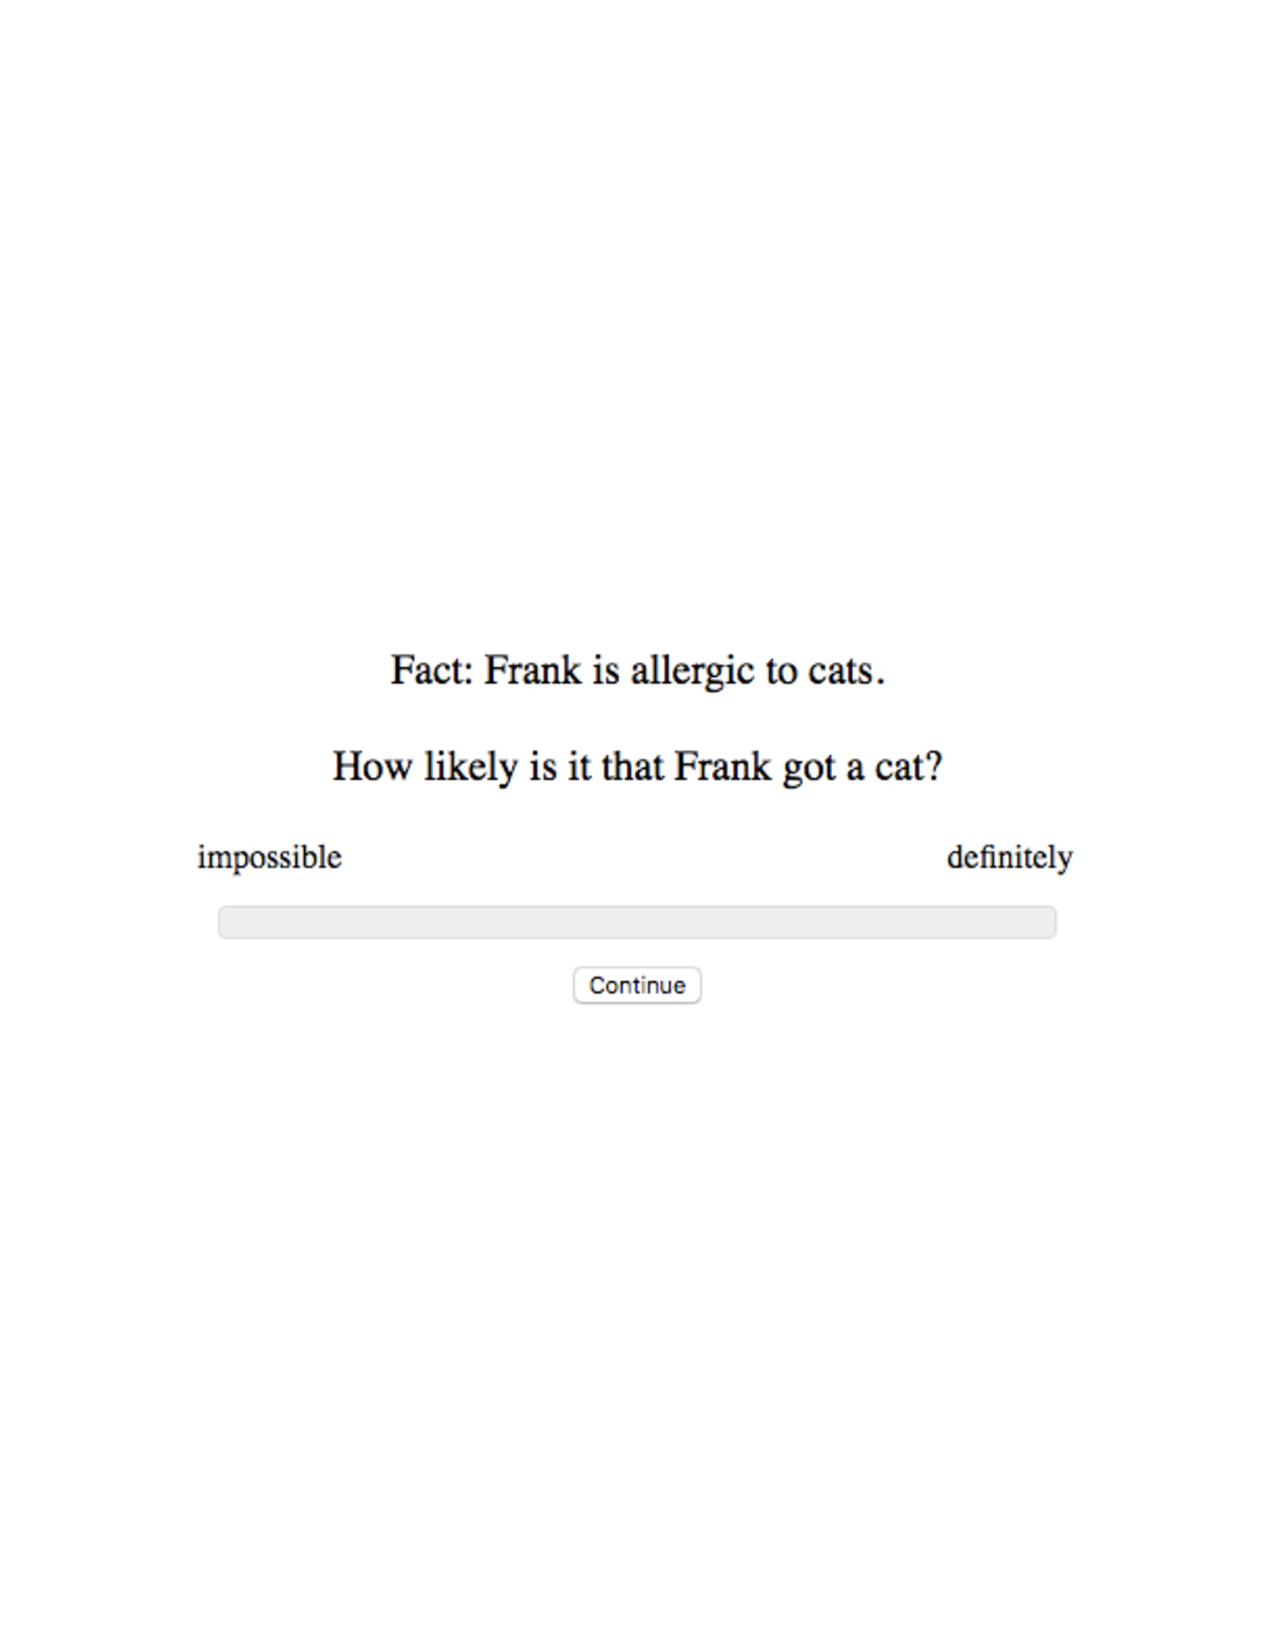
\includegraphics[width=8cm]{figures/exp1-trial}}
\end{center}
\caption{A sample trial in the prior probability norming study}\label{f-trial-exp1}
\end{figure}

After completing the experiment, participants filled out a short optional survey about their age, their gender, their native language(s) and, if English is their native language, whether they are a speaker of American English (as opposed to, e.g., Australian or Indian English). To encourage them to respond truthfully, participants were told that they would be paid no matter what answers they gave in the survey. 

\paragraph{Data exclusion}
Prior to analysis, the data from 8 participants who did not self-identify as native speakers of American English were excluded. For the remaining 87 participants, we inspected their responses to the two control stimuli; the group means were .86 for (\ref{control1}a) and .03 for (\ref{control1}b). 19 participants gave responses lower than .8 to (\ref{control1}a) or responses higher than .2 to (\ref{control1}b), suggesting that these participants did not attend to the task or interpreted the task differently. The data from these 19 participants were also excluded, leaving data from 68 participants (ages 21-75; median: 36; 31 female, 37 male).  


\subsection{Results and discussion}

As expected, the likeliness ratings of events were influenced by facts about the world: the mean prior probability of the events was .7 (sd = .21) when presented with facts that made the events more likely and .16 (sd = .17) when presented with facts that make the events less likely. Figure \ref{f-priors} shows the likeliness ratings for the 20 events given facts that make the events more likely (brown dots) and given the facts that make the events less likely (blue dots). Mean likeliness ratings for each of the 40 fact/event pairs are shown as black dots. Error bars indicate 95\% confidence intervals.

\begin{figure}
\centering

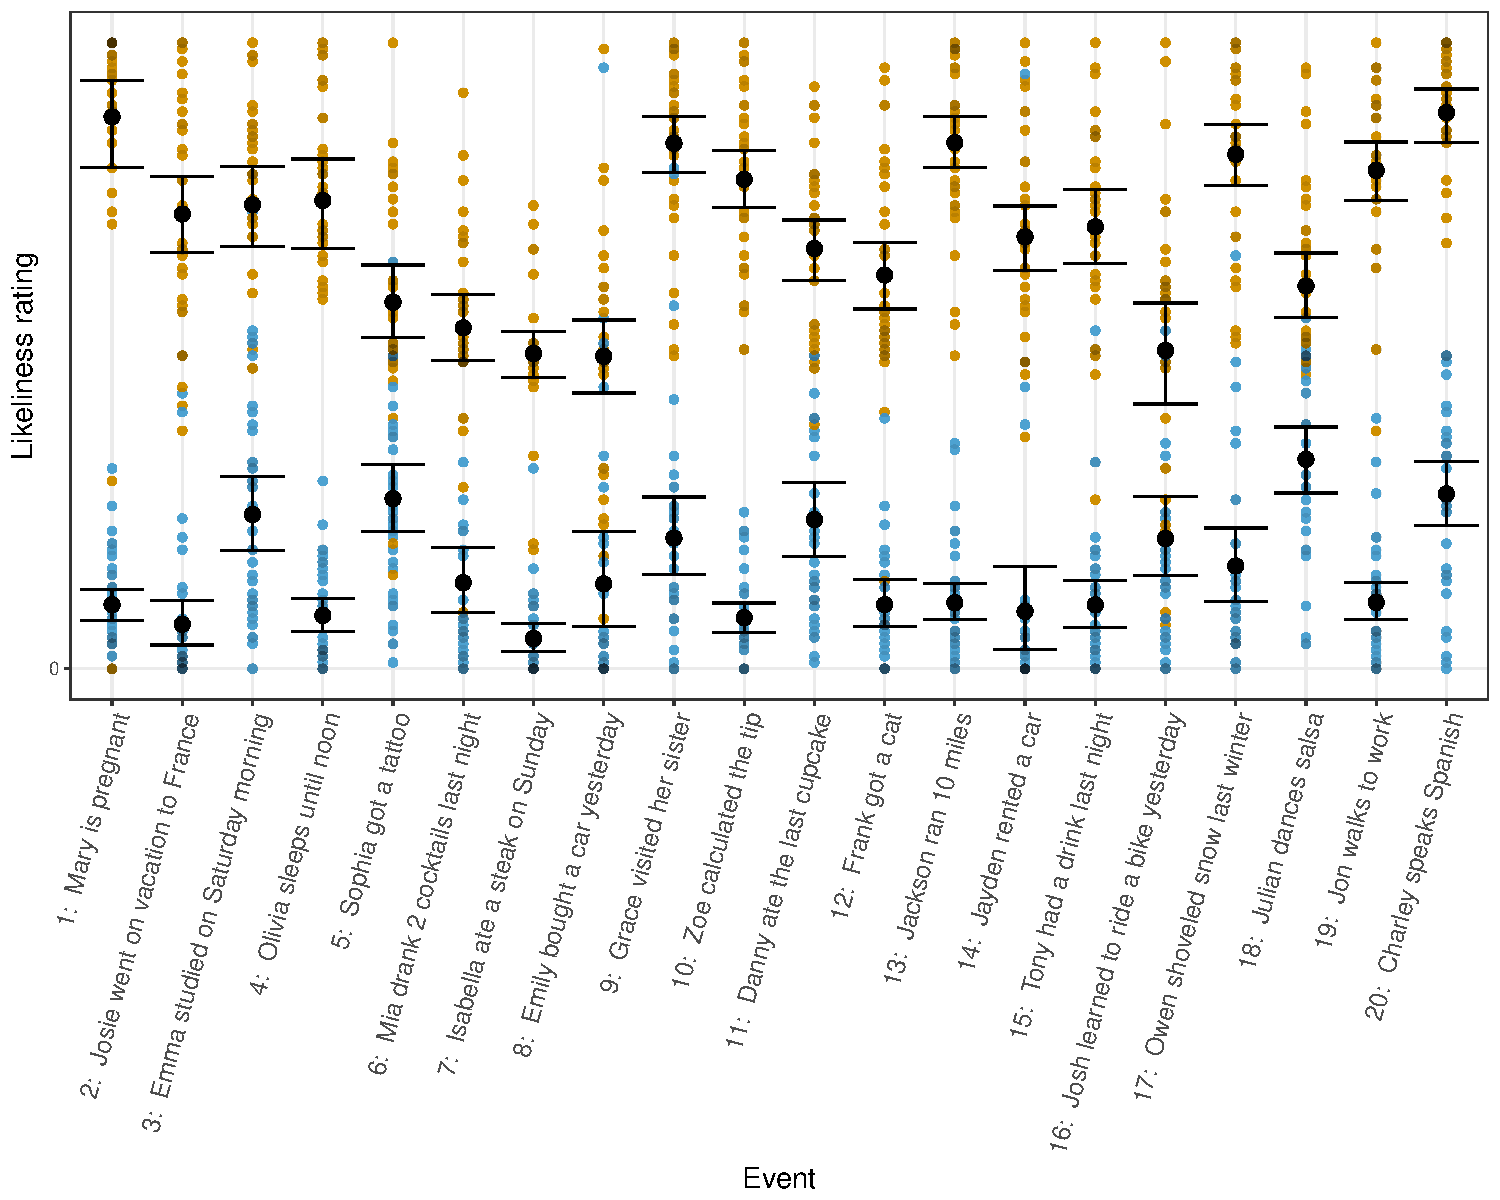
\includegraphics[width=.8\paperwidth]{../results/1-prior/graphs/target-ratings}

\caption{Likeliness ratings for 20 events given facts about the world that make the events more likely (brown dots) and facts about the world that make the events less likely (blue dots); darker dots indicate overlapping ratings. Mean likeliness ratings for the 40 fact/event pairs are given by black dots. Error bars indicate 95\% confidence intervals.}\label{f-priors}
\end{figure}

Figure \ref{f-priors} shows that, for each event, the likeliness of the event is higher given the fact that makes the event more likely than given the fact that makes the event less likely. The most likely event is that of Charley speaking Spanish given the fact that he lives in Mexico (mean: .89, sd: .14). The least likely event is that of Isabella eating a steak on Sunday given the fact that she is a vegetarian (mean: .05, sd: .07). Given that, for the 68 remaining participants, the mean prior probability of the control event in (\ref{control1}a) was .99 (sd: .01) and the mean prior probability of the control event in (\ref{control1}b) was .01 (sd: .01), we conclude that the likeliness of none of the 40 event/fact pairs is at ceiling or at floor.

\section{Control stimuli in Exp.~2}\label{a-exp2-control}

\begin{exe}
\ex\label{control2-complete}
\begin{xlist}

\ex {\bf Fact (which NAME knows):} Zack is a member of the golf club.
\\ {\bf NAME:} Is Zack coming to the meeting tomorrow?

\ex {\bf Fact (which NAME knows): Mary visited her aunt on Sunday} 
\\ {\bf NAME: Is Mary's aunt sick?} 

\ex {\bf Fact (which NAME knows): Todd goes to the gym 3 times a week} 
\\ {\bf NAME: Did Todd play football in high school?} 

\ex {\bf Fact (which NAME knows): Vanessa won a prize at school} 
\\ {\bf NAME: Is Vanessa good at math?} 

\ex {\bf Fact (which NAME knows): Trish sent Madison a card} 
\\ {\bf NAME: Did Madison have a baby?} 

\ex {\bf Fact (which NAME knows): Hendrick just bought a car} 
\\ {\bf NAME: Was Hendrick's car expensive?} 

\end{xlist}
\end{exe}

\section{Materials used in the event probability norming study}\label{a-exp1}

The list below provides the 20 English sentences that describe the events whose prior probability was explored in the norming study described in section \ref{s-norming}, together with the fact about the world that makes the event more likely and the fact about the world that make the event less likely.

\begin{enumerate}[leftmargin=3ex,itemsep=-2pt]
\item Mary is pregnant (Mary is a middle school student / Mary is taking a prenatal yoga class)
\item Josie went on vacation to France (Josie doesn't have a passport / Josie loves France)
\item Emma studied on Saturday morning (Emma is in first grade / Emma is in law school)
\item Olivia sleeps until noon (Olivia has two small children / Olivia works the third shift)
\item Sophia got a tattoo (Sophia is a high end fashion model / Sophia is a hipster)
\item Mia drank 2 cocktails last night (Mia is a nun / Mia is a college student)
\item Isabella ate a steak on Sunday (Isabella is a vegetarian / Isabella is from Argentina)
\item  Emily bought a car yesterday (Emily never has any money / Emily has been saving for a year)
\item  Grace visited her sister (Grace hates her sister / Grace loves her sister)
\item Zoe calculated the tip (Zoe is 5 years old / Zoe is a math major)
\item  Danny ate the last cupcake (Danny is a diabetic / Danny loves cake)
\item  Frank got a cat (Frank is allergic to cats / Frank has always wanted a pet)
\item  Jackson ran 10 miles (Jackson is obese / Jackson is training for a marathon)
\item  Jayden rented a car (Jayden doesn't have a driver's license / Jayden's car is in the shop)
\item  Tony had a drink last night (Tony has been sober for 20 years / Tony really likes to party with his friends)
\item  Josh learned to ride a bike yesterday (Josh is a 75-year old man / Josh is a 5-year old boy)
\item  Owen shoveled snow last winter (Owen lives in New Orleans / Owen lives in Chicago)
\item  Julian dances salsa (Julian is German / Julian is Cuban)
\item  Jon walks to work (Jon lives 10 miles away from work / Jon lives 2 blocks away from work)
\item  Charley speaks Spanish (Charley lives in Korea / Charley lives in Mexico)
\end{enumerate}

\clearpage


\section{Materials used in Exp 2}\label{a-exp2}

\section{Materials used in Exp 3}\label{a-exp3}

\bibliographystyle{cslipubs-natbib}
\bibliography{bibliography}


\end{document}
